\documentclass[
  final,
  babelLanguage=portuguese,
  % desktopVersion,
  %showtrims,
  %overleaf,
]{anecdote}

%\graphicspath{{./assets/photos/300dpi/}}
\graphicspath{{./assets/photos/92dpi/}}

\usepackage{local}

%% Details of the book
%% ===================

\title{A Palavra do Buddha}
\subtitle{}
\author{Nyanatiloka Mahāthera}
\publisher{Publicações Sumedhārāma}
\date{2024-02-10}
\editionInfo{\textit{Terceira edição portuguesa}, 2024}
\ISBN{000-000-0000-00-0}% TODO update ISBN

% === Metadata ===

\hypersetup{
  pdftitle={\thetitle},
  pdfauthor={\theauthor},
  pdfcopyright={Copyright (C) 2024, \thePublisher},
  pdfsubject={},% TODO subject
  pdfkeywords={},% TODO keywords
  pdflicenseurl={https://creativecommons.org/licenses/by-nc-nd/4.0/},
  pdfcontacturl={},
  pdflang={en},
}

% \pdfinfo{%
%   /Title (\thetitle)%
%   /Author (\theauthor)
%   /Subject (subject)% TODO subject
%   /Keywords (keywords)% TODO keywords
%   /GTS_PDFXVersion (PDF/X-1:2001)%
%   /GTS_PDFXConformance (PDF/X-1a:2001)%
% }

%% === Load further packages ===

%% === Hyphenation exceptions and corrections ===

\hyphenation{London akusala samudaya parinibbāna kammapatha kármicas dhammavicaya sambojjhaṅga aṭṭhangika}

\begin{document}

\frontmatter

\ifdesktopversion
\desktopCover{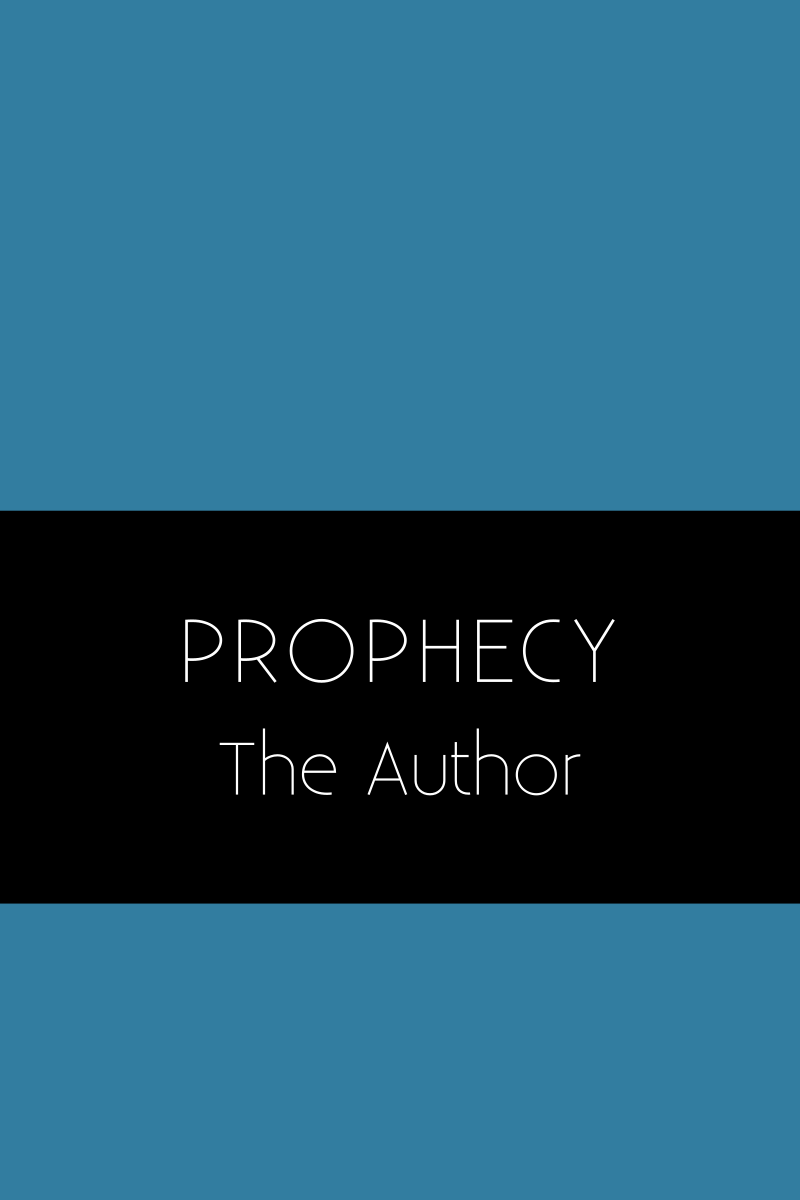
\includegraphics[height=\paperheight]{./desktop-cover.png}}
\fi

\cleartorecto
\thispagestyle{empty}
\vspace*{5em}

% FIXME: ? title style with large bold text

{\centering

\settowidth{\titleLength}{%
  {\Large\chapterTitleFont\scshape\MakeLowercase{\thetitle}}%
}

{\Large\chapterTitleFont\scshape\MakeLowercase{\thetitle}}\\[0.3\baselineskip]
\setlength{\xheight}{\heightof{X}}
\raisebox{0.5\xheight}{\color[gray]{0.4}\rule{\titleLength}{0.25pt}}\\[0.3\baselineskip]

Uma Síntese do Ensinamento do Buddha\\
baseada no Cânone Pāli

\vfill

Compilado, traduzido e comentado por

Nyanatiloka Mahāthera

% Tradução Portuguesa de Bhikkhu Dhammiko

\vspace*{5em}

}



\cleartoverso
\thispagestyle{empty}

{\copyrightsize
\centering
\setlength{\parindent}{0pt}%
\setlength{\parskip}{0.8\baselineskip}%

\thetitle\ -- \thesubtitle\\
por \theauthor

Publicações Sumedhārāma\\
\href{https://sumedharama.pt}{www.sumedharama.pt}

Para distribuição gratuita\\
\textit{Sabbadānaṁ dhammadānaṁ jinati}\\
‘A oferta de Dhamma é superior a qualquer outra oferta.’

Este livro encontra-se disponível para distribuição gratuita em:\\
\href{https://sumedharama.pt}{www.sumedharama.pt}

ISBN \theISBN

Copyright \copyright\ Publicações Sumedhārāma 2024

Tradução: Dhammiko Bhikkhu\\
Formatação: Gambhīro Bhikkhu

Traduzido do original `The Word of the Buddha'\\
Publicado por Buddhist Publication Society\\
Sangharaja Mawatha -- Kandy, Sri Lanka

16ª Edição 1981\\
17ª Edição 2001\\
1ª Edição Portuguesa 2010\\
2ª Edição Portuguesa 2013\\
3ª Edição Portuguesa 2024

\vfill

{\footnotesize

Este trabalho está licenciado com uma Licença Creative Commons\\
Atribuição-NãoComercial-SemDerivações 4.0 Internacional.

Veja página \pageref{copyright-details} para mais detalhes sobre direitos e restrições desta licença.\\
Produzido com o sistema tipográfico \LaTeX. Fonte utilizada:\\
EB Garamond, Crimson Roman e Open Sans.

\theEditionInfo

}}


\cleartorecto
\tableofcontents*

\chapter{Imagem da Capa}

\textbf{``Pegadas do Buddha'' (Buddhapada)} é uma das representações mais
antigas da arte e da simbologia budista na fase anti iconográfica (a ausência de
estátuas). O \emph{Buddhapada} é altamente reverenciado em países budistas,
especialmente no Sri Lanka e na Tailândia. Na Índia, os pés têm sido objecto de
respeito muito antes do Budismo, como arquétipo de ligação do ``transcendente''
à Terra.

De acordo com a lenda, o Buddha depois da sua iluminação, deixou a impressão dos
seus pés numa pedra onde caminhara em Kusinara, na Índia. As pegadas simbolizam
a \textbf{presença do Buddha}, no contacto com a Terra e paradoxalmente, também
a \textbf{ausência do Buddha}, aquando da sua entrada no Nirvāna, daí a memória
ao ideal budista do desapego.

As pegadas do Buddha são normalmente representadas com todos os dedos dos pés no
mesmo comprimento e com um \emph{Dharma-chakra} (Roda do \emph{Dharma}) ao
centro. Outros símbolos budistas antigos aparecem também nos calcanhares e
dedos, tais como o Lótus, a \emph{Swastika} e as \emph{Triratna} (Três Jóias).

Resgatando o verdadeiro significado ancestral da cruz \emph{swastika},
independentemente das atrocidades cometidas com a sua imagem pelos nazis, a
palavra deriva do Sânscrito \emph{svastika} (em Devanagari \devanagari{स्वस्तिक}),
significando fortuna e bem-estar, um símbolo utilizado para dar boa sorte. A
palavra é composta por su-significando ``bom'', ``bem'' e \emph{asti} ``ser''
\emph{svasti} significando ``bem-estar''. O sufixo - \emph{ka} ora forma um
diminutivo ora intensifica o significado verbal, e \emph{svastika} pode então
traduzir-se literalmente como ``aquilo que está associado com bem-estar'',
correspondendo a ``boa fortuna'' ou ``algo auspicioso''. Historicamente,
tornou-se um símbolo sagrado no Hinduísmo, Jainismo, Mitraismo e Xamanismo,
ganhando importância no Budismo durante o Império Máuria. Com a propagação do
Budismo, alcançou o Tibete e a China. Pensa-se que o seu uso pela fé indígena do
Tibete, bem como de religiões sincréticas como a \emph{Cao Dai} do Vietnam e a
\emph{Falun Gong} da China, também se originou do Budismo. O símbolo pode também
ser encontrado por toda a Coreia.

Hoje em dia é usado na arte e nas escrituras budistas, representando o
\emph{Dharma}, a harmonia universal e o equilíbrio dos opostos. Pode observar-se
a \emph{swastika} nos pilares de Ashoka (304 A.C.), onde simboliza a dança
cósmica em torno de um centro fixo, funcionando como protecção contra o mal.

\chapter{PREFÁCIO à Décima Primeira Edição Inglesa}

\emph{A Palavra do Buddha}, cuja primeira edição foi publicada em língua alemã, constituiu a primeira explanação sistemática das linhas mestras do Ensinamento do Buddha, apresentada pelas palavras do próprio Mestre, tal como encontradas no \emph{Sutta Piṭaka} do Cânone Pāḷi Budista.

Embora possa servir como primeira introdução para o principiante, o objectivo principal deste livro é oferecer ao leitor que já se encontra mais ou menos familiarizado com as ideias fundamentais do Budismo, uma síntese clara, autêntica e concisa dos seus diversos ensinamentos, no enquadramento das ``Quatro Nobres Verdades'', respectivamente as verdades do sofrimento (inerente a toda a existência), da origem do sofrimento, da extinção do sofrimento e do caminho que conduz à extinção do sofrimento. Verifica-se pelo próprio conteúdo do livro, como os ensinamentos do Buddha, em última análise, convergem todos para uma realização final: a Libertação do Sofrimento. Por essa razão se encontrava impressa na capa da primeira edição em alemão, a seguinte passagem do \emph{Aṅguttara Nikāya}, que diz:

\emph{``Eu ensino não só a verdade do sofrimento, como também a libertação desse sofrimento''.}

Os textos, traduzidos do Pāḷi original, foram seleccionados de entre as cinco grandes colecções de discursos que formam o \emph{Sutta Piṭaka}. Foram agrupados e explicados de modo a formarem um todo interligado. Assim, a colecção, originalmente compilada de entre os inúmeros e volumosos livros do \emph{Sutta Piṭaka} para orientação do próprio autor, revela-se um guia fidedigno para o estudante do Budismo. Facilita o trabalho, no sentido de consultar todas as demais secções das escrituras Pāḷi, permitindo obter uma visão clara no seu todo; poderá ajudar a relacionar a parte principal da doutrina com os inúmeros pormenores encontrados em estudos subsequentes.

Como o livro contém muitas definições e explanações de termos importantes da doutrina, com respectiva equivalência Pāḷi, pode, com a ajuda da pronúncia Pāḷi (p. 18), servir como uma referência útil para o estudo individual da doutrina do Buddha.

Depois da primeira edição em língua alemã em 1906, a primeira versão em língua inglesa foi publicada em 1907 e, desde então, já se fizeram mais dez, incluindo uma edição abreviada para estudantes (Colombo, 1948, Y.M.B.A.) e outra americana (Santa Bárbara, Cal., 1950, J. F. Rowny Press). A obra foi também incluída na Bíblia Budista de Dwight Goddard, publicada nos Estados Unidos da América.

Para além das edições subsequentes alemãs, já foram também editadas em francês, italiano, checo, finlandês, russo, japonês, hindu, bengali e cingalês. O Pāḷi original das passagens traduzidas foi publicado em caracteres ceilonenses (edição do autor, sob o título \emph{Sacca-Sangaha}, Colombo, 1914) e em escrita devanagárica na Índia.

A 11ª edição foi totalmente revista. Foram feitas algumas adições à Introdução e às notas explicativas, bem como acrescentados alguns textos.

\textbf{Nyanatiloka}

\chapter[Prefácio à Décima Quarta Edição Inglesa (1967)]{Prefácio\\ à Décima Quarta Edição Inglesa\\ (1967)}

O venerável autor desta pequena obra emblemática da literatura budista, faleceu
em 28 de Maio de 1957, com a idade de 79 anos. A presente edição comemora o
décimo aniversário da sua morte.

Antes da sua partida, foi incluída uma reedição revista deste livro como 12ª
edição, em \emph{``The Path of Buddhism''}, publicação do Buddhist Council of
Ceylon (Lanka Bauddha Mandalaya). O texto das reimpressões seguintes foi baseado
nessa 12ª edição, apenas com algumas emendas menores. A partir da 13ª edição
(1959) e com a gentil permissão dos primeiros editores ``Sāsanadhāra Kantha
Samitiya'', o livro é publicado agora pela Buddhist Publication Society
(Sociedade de Publicações Budistas).

Paralelamente a esta edição, a Sociedade publica também, em letra romana, com o
título de \emph{Buddha Vacanaṁ}, os textos Pāli originais que estão traduzidos
no presente livro. Esta edição Pāli tem o propósito de servir como leitura para
estudantes de língua Pāli e como manual de referência, bem como de breviário de
apreciação contemplativa para aqueles que, de certa forma, já conhecem a
linguagem das escrituras Budistas.

\bigskip

{\raggedleft
  Buddhist Publication Society\\
  Kandy, Ceylon, Dezembro 1967
\par}

\chapter{PREFÁCIO à Primeira Edição Portuguesa de 2010}

A compilação dos ensinamentos básicos dos Suttas do Tripitaka, pelo Venerável Nyanatiloka, tem sido a minha referência e guia de meditação ao longo de 44 anos de prática monástica.

No primeiro ano da minha vida monástica, em 1966, usei ``\emph{A Palavra do Buddha}'' como único suporte durante esse longo e intenso ano de retiro de meditação em Wat Nern Panow, Nong Khai, Tailândia. Esse ano transformou a minha vida e deu-me a inabalável fé na prática e no ensinamento do Buddha.

Estou muito feliz por termos este livro tão importante traduzido para a língua portuguesa. Que seja de grande benefício para todos aqueles que estão interessados nos ensinamentos essenciais do Senhor Buddha.

\textbf{Ven. Ajahn Sumedho}

Amaravati Buddhist Monastery

\chapter[Prefácio à Segunda Edição Portuguesa (2013)]{Prefácio\\ à Segunda Edição Portuguesa\\ (2013)}

Uma tradução é sempre delicada no que respeita a preservar o sentido e
significado original que o autor quis transmitir, principalmente quando envolve
um Ensinamento milenar, como o do Buddha. Este livro em particular, inclui
transcrições directas das Escrituras Budistas Theravada, sendo esta uma tradução
para a língua portuguesa da versão inglesa anteriormente traduzida do original
alemão. Por conseguinte, exigiu um cuidado extra com relação aos princípios
fundamentais do Dhamma, no sentido de evitar deturpações do seu significado
original, uma vez que contém precisamente transcrições directas parciais de
alguns dos principais \emph{Suttas} do Cânone Pāli.

Após várias considerações, procedeu"-se ao ajuste de alguns dos termos chave do
Budismo, como o caso mais pertinente do termo \emph{Sati} na língua Pāli,
traduzido normalmente para o inglês como “mindfulness” e para o português
directamente do inglês como “plena atenção”, não fazendo a justiça devida ao
significado original mais amplo que o termo \emph{Sati} comporta. Neste trabalho,
para melhor traduzir esse significado que comporta a descriminação e memória do 
que se aprendeu do bem e do mal, do que é saudável e nefasto (kusala e akusala),
decidiu"-se então adoptar a palavra “consciência” em vez de meramente “plena
atenção”, evitando assim a deturpação e o reducionismo do seu significado. De
uma forma mais abrangente, o termo português “consciência”, abarca
simultaneamente os quatro termos em inglês, “consciousness”, “conscience”,
“mindfulness” e “awareness”, que traduzem mais completamente as noções
ausentes nos termos “plena atenção” de uma consciência já espiritual, não só
de atenção mesmo que plena no seu limite cognitivo em termos de memória,
inteligência e consciência - a presença e lembrança correcta do que é importante
e se deve fazer e como se deve fazer, saudável e correctamente, diligentemente,
com responsabilidade humana e espiritual. Significa a forma cuidada com que se
usa, aplica e presta atenção, mais do que a atenção propriamente dita, que por
si só, na óptica da Palavra do Buddha, pode ser aplicada e usada tanto sábia e 
conscientemente como néscia e inconscientemente, até de uma forma criminosa. 
Daí os termos \emph{yoniso manasikāra} (atenção correcta, sabiamente aplicada) 
versus \emph{ayoniso manasikāra} (atenção incorrecta, mal aplicada).

Por sua vez na cultura e língua inglesa, o uso dos termos “Consciousness”
versus “Conscience” apresentam uma distinção de significado em que o
significado o primeiro se circunscreve mais aos sentidos físicos humanos, a
função cognitiva física e sensorial do corpo, que em Pāli se traduz por
\emph{Viññāṇa}, termo que neste livro se traduziu para o português como
“cognição”, fazendo aqui também jus à raiz sânscrita do Pāli \emph{Viññāṇa}.
“Conscience” na cultura e língua inglesa, traduz mais o aspecto ético que se
aproxima mais do significado de \emph{sati} no que respeita ao princípio do
cuidado, da diligência e da consciência, num todo de princípios éticos e
qualidades fundamentais que no Ensinamento do Buddha ajudam a conduzir"-nos ao
caminho da purificação e realização espiritual.

Sendo este só um exemplo, entre vários termos, tentou"-se assim ajustar da melhor
forma as diferentes expressões usadas, no sentido de respeitar tanto o Pāli
original, como o próprio autor, o Venerável Nyanatiloka Mahāthera.

Os trechos em itálico Sans Serif encontrados ao longo do livro, são os comentários
do autor, à excepção dos termos Pāli também em itálico.

A fundamentação dos significados Pāli, foi apoiada com a colaboração de outros
monásticos versados em Pāli e com o suporte adicional dos dicionários
‘Pāli"-English Dictionary’ de T. W. Rhys Davids e William Stede, bem como
‘Buddhist Dictionary’ de Nyanatiloka Mahāthera.

\bigskip

{\raggedleft
  Dhammiko Bhikkhu\\
  2013
\par}

\chapter{Abreviaturas}

DN -- \emph{Dīgha Nikāya}

MN -- \emph{Majjhima-Nikāya}

AN -- \emph{Aṅguttara-Nikāya}

SN -- \emph{Saṁyutta-Nikāya}

Dhp -- \emph{Dhammapada}

Ud -- \emph{Udāna}

Snp -- \emph{Sutta-Nipāta}

VisM. -- \emph{Visuddhi-Magga (A Senda da Purificação)}

B. Dict. -- \emph{Buddhist Dictionary (Dicionário Budista)},\\
por Nyanatiloka Mahāthera

Fund. -- \emph{Fundamentals of Buddhism (Fundamentos do Budismo)},\\
por Nyanatiloka Mahāthera

\chapter{A Pronúncia Pāli}

\subsection{As Vogais}

FIXME add more examples

\textbf{a} -- Em Português é pronunciado como `\emph{a}' mudo em `par\prul{a}' ou `c\prul{a}nec\prul{a}'.

Em Português do Brasil é melhor exemplificar em inglês: O `\emph{a}' funciona como o `\emph{u}' na palavra inglesa `\emph{shut}'; nunca aberto como em `\emph{cat}', e nunca como em `\emph{take}'.

\emph{ā} -- Como `á' de `já'ou `a' de `tomar'.

\emph{e} -- É pronunciado como `ê' longo.

\emph{i} -- Como `\emph{i}'.

\emph{ī} -- Como `\emph{i}' longo.

\emph{o} -- Como `\emph{ô}' longo.

\emph{u} -- Como `\emph{u}'.

\emph{ū} -- Como `\emph{u}' longo.

\subsection{As Consoantes}

\emph{c} -- É pronunciado como `\emph{tch}', assim como o `\emph{ch}' inglês em `\emph{chair}'; nunca como `\emph{c}' em `\emph{cavalo}' ou `\emph{ch}' em `\emph{cheirar}', `\emph{chover}'.

\emph{g} -- Como em `\emph{gamo}'.

\emph{h} -- Mesmo que colocado imediatamente a seguir às consoantes ou consoantes duplas, o `\emph{h}' é sempre aspirado como sopro em suspiro gutural, típico na língua inglesa; exemplo como no inglês: `\emph{bh}' `\emph{cabhorse}'; `\emph{ch}' como

`\emph{chh}' em `\emph{ranch-house}'; `\emph{dh}' como em `\emph{handhold}'; `\emph{gh}' como em `\emph{bag-handle}'; `\emph{jh}' como `\emph{dgeh}' em `\emph{sledgehammer}', etc.

\emph{j} -- Não como em `\emph{jarra}', mas como `\emph{dj}' de `\emph{djarra}'; como na palavra inglesa `\emph{joy}'.

\emph{ṁ} -- O chamado `nasal' é como o `m' em `\emph{amparo}' ou, `\emph{ambiente}'.

\emph{s} -- Sempre como em `\emph{sublimar}' ou em `\emph{se}'; nunca como `\emph{z}', ex: em `\emph{causar}' ou em `\emph{físico}'.

\emph{ñ} -- Como o `\emph{nh}' normal na língua portuguesa; ex: `\emph{manhã}', `\emph{minha}', `\emph{apanhar}', etc.

\emph{ph} -- Como `\emph{f}' seguido de suspiro gutural como no inglês, assim como o `\emph{ph}' da palavra inglesa `\emph{haphazard}'.

\emph{th} -- Como `\emph{t}' seguido de suspiro gutural típico do `\emph{h}' em inglês.

\emph{y} -- Como o `\emph{i}' normal.

\emph{ṭ, ṭh, ḍ, ḍh} -- São sons de língua, ditos cerebrais; ao pronunciá-los deve-se pressionar a língua contra o céu da boca.

\emph{Consoantes duplas} -- Cada uma deve ser pronunciada, como `\emph{bb}' em `\emph{subbase}'.

\chapter{Introdução}

\section{O Buddha}

O Buddha ou Iluminado -- lit. Aquele que sabe ou o Desperto -- é o nome
honorífico conferido ao Sábio indiano, Gotama, que desvendou e proclamou ao
mundo a lei da libertação, conhecida no Ocidente pelo nome de Budismo.

Nasceu no Século VI a.C., em Kapilavatthu, filho do rei que na época regia o
País Sakya, um principado situado na zona de fronteira com o actual Nepal. O seu
nome próprio era Siddhattha e seu nome de clã Gotama (Sânscrito:
\emph{Siddhārtha Gautama}). Aos 29 anos de idade, renunciou ao esplendor da sua
vida principesca como herdeiro real, e tornou"-se um asceta mendicante, com o
propósito de descobrir uma solução para aquilo que antes havia reconhecido como
um mundo de sofrimento. Depois de uma busca de seis anos sob a orientação de
vários instrutores religiosos e de um período de auto"-mortificação infrutífera,
Siddhattha finalmente alcançou a Iluminação Perfeita (\emph{sammāsambodhi}),
debaixo da árvore \emph{Bodhi} em Gayā (actualmente Boddh"-Gayā). Seguiram"-se
quarenta e cinco anos de incansável ensinamento e pregação, e finalmente, no seu
octogésimo ano de vida, morre em Kusinara ``aquele ser não iludido que surgiu
para a bênção e alegria do mundo''.

O Buddha não é nem um deus nem um profeta, nem a encarnação de um deus, mas um
ser humano supremo que, através do seu próprio empenho, alcançou a redenção
final, a sabedoria perfeita, tornando"-se ``o mestre sem par de deuses e
homens''. É um ``Salvador'' unicamente no sentido em que mostra aos homens como
se salvarem a si próprios, seguindo até ao fim, na prática, o caminho percorrido
e mostrado por ele. O Buddha, na sua consumada harmonia de sabedoria e
compaixão, encarna o ideal universal e intemporal do homem Aperfeiçoado.

\section{O Dhamma}

O Dhamma -- é o Ensinamento da Libertação total, tal como foi desvendado, realizado e proclamado pelo Buddha. Tem sido transmitido na antiga língua Pāli e preservado em três grandes colecções de livros, chamados \emph{Ti"-Piṭaka}, os ``Três Cestos'', nomeadamente:

\begin{enumerate}
  \item o \emph{Vinaya"-piṭaka}, ou a Colecção da Disciplina, contendo as regras
        da ordem monástica;

  \item o \emph{Sutta"-piṭaka}, ou a Colecção dos Discursos, consistindo em
        vários livros de discursos, diálogos, versos, histórias, etc., tratando
        da doutrina em si, tal como foi resumida nas ``Quatro Nobres Verdades'';

  \item o \emph{Abhidhamma"-piṭaka}, ou a Colecção Filosófica, apresentando os
        ensinamentos do \emph{Sutta"-piṭaka} de uma forma sistemática e
        filosófica.
\end{enumerate}

O Dhamma não é uma doutrina de revelação, mas o ensinamento da Iluminação
baseado na compreensão lúcida da realidade. É~o~ensinamento da \emph{Quádrupla
  Verdade} que trata dos factos fundamentais da vida e da libertação realizada
através do próprio esforço do homem, em direcção à introspecção e purificação. O
Dhamma oferece um sistema ético superior, mas realista, uma análise
penetrante da vida, uma filosofia profunda, métodos práticos para o treino da
mente -- resumidamente, uma orientação no seu todo, perfeita e acessível no
Caminho para a Libertação. Ao responder ao clamor tanto do coração como da
razão, e ao mostrar o libertador ``Caminho do Meio'' que nos conduz para além de
todos os extremos fúteis e destruidores da mente e da conduta individual, o
Dhamma tem e terá sempre um apelo intemporal e universal onde quer que
existam corações e mentes suficientemente maduras para valorizar a sua Mensagem.

\section{O Sangha}

O Sangha -- lit. a assembleia, ou comunidade -- é a Ordem dos \emph{Bhikkhus} ou
Monges Mendicantes, fundada pelo Buddha e ainda existente na sua forma original
em Myanmar (Birmânia), Tailândia, Sri Lanka (Ceilão), Camboja, Laos e Chittagong
(Bengala). Juntamente com a Ordem dos monges Jainas, é uma das ordens monásticas
mais antigas do mundo. Entre os mais famosos discípulos no tempo do Buddha,
encontravam"-se: Sāriputta que, a seguir ao próprio Mestre, tinha a mais profunda
compreensão no Dhamma; Moggallāna, dotado com os maiores poderes
\mbox{sobrenaturais}; Ānanda, o devotado discípulo e constante companheiro do Buddha;
Mahā"-Kassapa, o Presidente do Conselho que se reuniu em Rājagaha imediatamente a
seguir à morte do Buddha; Anuruddha, o mestre de visão divina e da consciência
pura e Rāhula, o filho do próprio Buddha.

O Sangha providencia o veículo externo e as condições favoráveis para
todos aqueles que, livres das distracções mundanas, desejem seriamente devotar
toda a sua vida à realização do mais elevado objectivo que é a libertação.
Assim, o Sangha também possui um significado universal e intemporal, onde
quer que o desenvolvimento religioso alcance a maturidade.

\section{O Triplo Refúgio}

O Buddha, o Dhamma e o Sangha, são designados ``As Três Jóias''
(\emph{tiratana}) pela sua pureza inigualável e por serem, para o budista,
aquilo que há de mais precioso no mundo. Estas ``Três Jóias'' constituem também
o ``Triplo Refúgio'' (\emph{ti"-saraṇa}) que o praticante assume, ao proferir as
palavras com as quais o declara ou reafirma, ao adoptá"-las como guias da sua
vida e do seu pensamento.

A fórmula Pāli do Refúgio é ainda a mesma aquando do tempo do Buddha:

\begin{verse}
  \emph{Buddhaṁ saraṇaṁ gacchāmi.}\\
  \emph{Dhammaṁ saraṇaṁ gacchāmi.}\\
  \emph{Sanghaṁ saraṇaṁ gacchāmi.}

  Eu busco o refúgio no Buddha.\\
  Eu busco o refúgio no Dhamma.\\
  Eu busco o refúgio no Sangha.
\end{verse}

É através do simples acto de recitar esta fórmula três vezes, que uma pessoa se
considera budista. Na segunda e terceira repetições, acrescentam"-se as palavras
correspondentes \emph{Dutiyampi} e \emph{Tatiyampi} no início das frases:

\begin{verse}
  \emph{Dutiyampi Buddhaṁ saraṇaṁ gacchāmi}.\\
  \emph{Dutiyampi Dhammaṁ saraṇaṁ gacchāmi.}\\
  \emph{Dutiyampi Sanghaṁ saraṇaṁ gacchāmi.}

  Pela 2ª vez eu busco o refúgio no Buddha.\\
  Pela 2ª vez eu busco o refúgio no Dhamma.\\
  Pela 2ª vez eu busco o refúgio no Sangha.

  \emph{Tatiyampi Buddhaṁ saraṇaṁ gacchāmi.}\\
  \emph{Tatiyampi Dhammaṁ saraṇaṁ gacchāmi.}\\
  \emph{Tatiyampi Sanghaṁ saraṇaṁ gacchāmi.}

  Pela 3ª vez eu busco o refúgio no Buddha.\\
  Pela 3ª vez eu busco o refúgio no Dhamma.\\
  Pela 3ª vez eu busco o refúgio no Sangha.
\end{verse}

\section{Os Cinco Preceitos}

A seguir à fórmula do Triplo Refúgio, normalmente assumem"-se os Cinco Preceitos
Morais (\emph{pañca"-sīla}). A sua observância é o requisito de base para uma
vida íntegra e consequente progresso em direcção à Libertação.

\begin{enumerate}
  \item \emph{Pāṇātipātā veramaṇī sikkhāpadaṁ samādiyāmi.}\\
        Eu assumo o preceito de me abster de matar seres vivos.

  \item \emph{Adinnādānā veramaṇī sikkhāpadaṁ samādiyāmi.}\\
        Eu assumo o preceito de me abster de tirar o que não me é oferecido.

  \item \emph{Kāmesu micchācārā veramaṇī sikkhāpadaṁ samādiyāmi.}\\
        Eu assumo o preceito de me abster de sexualidade imprópria.

  \item \emph{Musāvādā veramaṇī sikkhāpadaṁ samādiyāmi.}\\
        Eu assumo o preceito de me abster de discurso desonesto.

  \item \emph{Surāmeraya"-majja"-pamādaṭṭhānā veramaṇī sikkhāpadaṁ samādiyāmi.}\\
        Eu assumo o preceito de me abster de bebidas e drogas intoxicantes que
        conduzem à falta de consciência.
\end{enumerate}

\chapter{As Quatro Nobres Verdades}

Assim foi dito pelo Buddha, o Iluminado:

Foi por não compreender, por não realizar quatro coisas, que eu, discípulos, tal
como vós, tive de vaguear tanto tempo neste ciclo de renascimentos. E quais são
essas quatro coisas? São:

\begin{enumerate}
  \item A nobre verdade do sofrimento \emph{(dukkha)};

  \item A nobre verdade da origem do sofrimento (\emph{dukkha-samudaya});

  \item A nobre verdade da extinção do sofrimento (\emph{dukkha-nirodha});

  \item A nobre verdade do caminho que conduz à extinção do sofrimento (\emph{dukkha-nirodha-gāmini-paṭipadā}).
\end{enumerate}

\quoteRef{DN 16}

Enquanto a visão introspectiva e o conhecimento perfeitamente verazes,
respeitando estas ``Quatro Nobres Verdades'', não se clarificaram em mim de
forma alguma, durante esse tempo, não tive a certeza de ter conquistado a
suprema iluminação, insuperável em todo o mundo com os seus seres celestiais,
espíritos malignos e deuses, entre todas as hostes de ascetas, sacerdotes e
homens. Mas, assim que a visão introspectiva e o conhecimento perfeitamente
verazes, com respeito a estas ``Quatro Nobres Verdades'', se clarificaram em
mim, surgiu-me interior- mente a certeza de ter conquistado aquela suprema e
insuperável iluminação.

\quoteRef{SN 56.11}

E eu descobri aquela verdade profunda, tão difícil de perceber, difícil de
compreender, tranquilizadora e sublime, que não é conquistada por mero
raciocínio e só é visível aos sábios.

\quoteRef{MN 26}

O mundo, está, no entanto, votado ao prazer, deleitado no prazer, enfeitiçado
com o prazer. Na verdade, tais seres dificilmente compreenderão a lei da
condicionalidade, a génese dependente (\emph{paṭicca-samuppāda}) de tudo;
incompreensível para eles será também o fim de todas as formações, o abandono de
tudo o que subjaz a cada renascimento, o desaparecimento da cobiça, do desapego
-- a libertação, o \emph{Nibbāna}.

No entanto, existem seres cujos olhos estão só ligeiramente cobertos de poeira:
estes compreenderão a verdade.

\quoteRef{MN 26}


% Page 1 is the first page of the first chapter.
\mainmatter

\chapter{A Primeira Nobre Verdade}

\textbf{A Nobre Verdade do Sofrimento}

\begin{quote}
O que é afinal a nobre verdade do sofrimento?

Nascer é sofrimento; envelhecer é sofrimento; morrer é sofrimento; a tristeza, a lamentação, a dor, a angústia e o desespero são sofrimento; não conseguir o que se deseja, é sofrimento; resumindo: os cinco agregados da existência são sofrimento.

E afinal, o que é nascer? É o aparecer de seres pertencentes a determinada ordem, a sua concepção e o acto de nascerem, o virem à existência, a manifestação dos agregados da existência, o começo da actividade sensitiva - a isto chama-se nascer.

E o que é envelhecer? É a degradação de seres pertencentes a determinada ordem, o acumular de mais idade, o debilitar, o ficar grisalho, o enrugar; a diminuição da força vital, a exaustão dos sentidos - a isto chama-se envelhecer.

E o que é morrer? É a partida e o desfalecer de seres de determinada ordem, a sua destruição, o desaparecimento, o término do seu período de vida, a dissolução dos agregados da existência, o descartar do corpo -- a isto chama-se morte.

E o que é a tristeza? A tristeza surge por qualquer tipo de perda ou infortúnio com que a pessoa se depara, pela preocupação, susto, aflição e lamento - a isto chama-se tristeza.

E o que é o lamento? É toda a lamúria e queixume por qualquer tipo de perda, infortúnio sofrido, o facto de se lamentar e recriminar, o estado de aflição e deploração - a isto chama-se

lamentação.
\end{quote}

D. 22

\begin{quote}
E o que é a dor? É a sensação dolorosa e desagradável produzida pela impressão física - a isto chama-se dor.

E o que é a angústia? É a dor e o desagrado mental, o sentimento doloroso e desagradável produzido pela impressão mental - a isto chama-se angústia.

E o que é o desespero? É o estado aflitivo e angustiante que surge de qualquer tipo de perda ou infortúnio com que a pessoa se depara, a desolação e a exasperação - a isto chama-se desespero.

E o que é o sofrimento por não se conseguir o que se deseja? Aos seres que estão sujeitos a nascer, surge o desejo: ``Ah, pudéssemos não estar sujeitos a nascer! Pudéssemos não ter pela frente mais nenhum nascimento!''. Sujeitos ao envelhecer, à doença, à morte, à tristeza, à lamentação, à dor, à angústia e ao desespero, surge-lhes o desejo: ``Ah, pudéssemos não estar sujeitos a estas coisas! Pudéssemos não ter de nos sujeitar a isto de novo!'' Mas tal não se obtém por mero desejo; e não obter o que se deseja, é sofrimento.

OS CINCO \emph{KHANDHAS}, OU AGREGADOS DA EXISTÊNCIA

\emph{(pañcupādānakkhandhā)}

E o que são os cinco agregados da existência? Eles são a corporalidade, a sensação, a percepção, as formações mentais e a cognição.

D. 22

Todos os fenómenos físicos, sejam eles do passado, do presente ou futuro, de uma pessoa ou exteriores a ela, grosseiros ou subtis, superiores ou inferiores, distantes ou próximos, pertencem ao agregado da corporalidade; todas as sensações pertencem ao agregado da sensação; todas as percepções pertencem ao agregado da percepção; todas as formações mentais pertencem ao agregado das formações mentais; toda a cognição pertence ao agregado da cognição.

M. 109

\emph{Estes agregados estão reunidos numa classificação quíntupla, na qual o Buddha resumiu todos os fenómenos físicos e mentais da existência, principalmente aqueles que parecem ao homem ignorante como sendo o seu ego e sua personalidade. Assim, o nascimento, o envelhecimento, a morte, etc., estão também incluídos nestes cinco agregados que na realidade englobam o mundo inteiro.}

O AGREGADO DA CORPORALIDADE

\emph{(rūpa-khandha)}

Afinal, o que é o agregado da corporalidade? São os quatro elementos primários e a corporalidade que deles deriva.

\textbf{Os Quatro Elementos}

E o que são os quatro elementos primários? São o elemento sólido, o elemento fluido, o elemento térmico e o elemento vibrante (ventoso).
\end{quote}

M. 28

\begin{quote}
\emph{Os quatro elementos (dhātu ou mahā-bhūta), popularmente chamados de Terra, Água, Fogo e Ar, deverão ser entendidos como qualidades elementares da matéria. São chamados em Pāḷi, paṭhavī-dhātu, āpo-dhātu, tejo-dhātu, vāyo-dhātu, e podem ser traduzidos como inércia, coesão, radiação e vibração. Todos os quatro estão presentes em qualquer objecto material, variando, no entanto, em grau de força. Se, por exemplo, o elemento Terra predomina, o objecto material é chamado ``sólido'', etc.}

\emph{A ``corporalidade derivada dos quatro elementos'' (upādāya rūpa ou upādā rūpa) consiste, conforme o Abhidhamma, nos seguintes vinte e quatro fenómenos e qualidades materiais: olho, ouvido, nariz, língua, corpo, forma visível, som, cheiro, sabor, masculinidade, feminilidade, vitalidade, a base física da mente (hadaya-vatthu; ver B. Dic.), gesto, fala, espaço (cavidades do ouvido, nariz, etc.), envelhecimento, mudança e nutrição.}

\emph{As impressões corporais (phoṭṭhabba -- o tacto) não são propriamente mencionadas entre estes vinte e quatro fenómenos, uma vez que são idênticas aos elementos, sólido, térmico e vibrante, que são apreendidas pelas sensações de pressão, frio, calor, dor, etc.}

1. O que é afinal o elemento sólido (\emph{paṭhavī-dhātu})? O elemento sólido pode ser do próprio indivíduo, ou pode ser exterior. E o que é o elemento sólido do indivíduo? O que quer que exista na própria pessoa ou no corpo de dureza e firmeza adquiridas karmicamente, tais como os cabelos da cabeça e do corpo, unhas, dentes, pele, carne, tendões, ossos, medula, rins, coração, fígado, diafragma, baço, pulmões, estômago, intestinos, mesentério, excremento e por aí fora -- a isto chama-se elemento sólido do indivíduo. Quer o elemento sólido seja do indivíduo ou do exterior, é meramente o elemento sólido.

E há que compreender que, de acordo com a realidade e a verdadeira sabedoria -- ``Isto não me pertence; eu não sou isto; isto não é o que eu sou''.

2. O que é afinal o elemento fluido (\emph{āpo-dhātu})? O elemento fluido pode ser do indivíduo ou do exterior. E o que é o elemento fluido do indivíduo? O que quer que exista na própria pessoa ou no corpo, de liquidez ou fluidez adquiridas karmicamente, tais como a bílis, mucosidades, pus, sangue, suor, gordura, lágrimas, gordura da pele, saliva, muco nasal, líquido nas articulações, urina e por aí fora -- a isto chama-se elemento fluido do indivíduo. Quer o elemento fluido seja do indivíduo ou do exterior, é mera- mente o elemento fluido.

E uma pessoa devia compreender, conforme a realidade e a verdadeira sabedoria, que: - ``Isto não me pertence; isto não sou eu; isto não é o que eu sou''.

3. O que é afinal o elemento térmico (\emph{tejo-dhātu})? O elemento térmico pode ser do indivíduo, ou do exterior. E o que é o elemento térmico do indivíduo? O que quer que exista na própria pessoa ou no corpo, de calor ou ardor adquiridos karmicamente, tal como tudo com que um indivíduo se aquece, consome, queima, e tudo através do qual digere o que foi ingerido, bebido, mastigado ou degustado e por aí adiante -- a isto chama-se o elemento térmico do indivíduo. Quer o elemento térmico seja do indivíduo ou do exterior, é meramente o elemento térmico.

Há que compreender, que de acordo com a realidade e a verdadeira sabedoria -- ``Isto não me pertence; eu não sou isto; isto não é o que eu sou''.

4. O que é afinal o elemento vibrante (ventoso) \emph{(vāyo-dhātu)}? O elemento vibrante pode ser do indivíduo, ou do exterior. E o que é o elemento vibrante do indivíduo? O que quer que exista na própria pessoa ou no corpo, de vento ou ventosidade adquiridos karmicamente, tal como os ventos que sobem e descem, os ventos do estômago e intestinos, o vento que permeia todos os membros, a inspiração e a expiração, etc. -- a isto chama-se o elemento vibrante do indivíduo. Quer o elemento vibrante seja do indivíduo ou do exterior, é meramente o elemento vibrante.

E há que compreender, conforme a realidade e a verdadeira sabedoria -- ``Isto não me pertence; eu não sou isto; isto não é o que eu sou''.

Assim como se chama ``cabana'' ao espaço circunscrito formado com madeira e juncos, canas e barro, da mesma forma se chama ``corpo'' ao espaço circunscrito formado com ossos, tendões, carne e pele.
\end{quote}

M. 28

\begin{quote}
O AGREGADO DA SENSAÇÃO

\emph{(vedanā-khandha)}

Existem três tipos de sensação: agradável, desagradável e nem agradável nem desagradável.

S. 36:1

O AGREGADO DA PERCEPÇÃO

\emph{(saññā-khandha)}

O que é afinal a percepção? Existem seis classes de percepção: percepção das formas, dos sons, odores, sabores, sensações físicas, e dos objectos mentais.

O AGREGADO DAS FORMAÇÕES MENTAIS

\emph{(sankhāra-khandha)}

O que são afinal as formações mentais? Existem seis classes de volições (\emph{cetanā}): vontade projectada nas formas (\emph{rūpa-sañcetanā}), nos sons, odores, sabores, nas sensações físicas, e nos objectos mentais.

S. 22:56

\emph{O ``agregado das formações mentais'' (saṇkhāra-khandha), é um termo colectivo para representar inúmeras funções ou aspectos da actividade mental que, acrescidos à sensação e à percepção, estão presentes num só momento da consciência. No Abhidhamma, são distinguidas cinquenta formações mentais, sete das quais são factores constantes da mente. O número e a composição do restante, varia consoante o carácter da respectiva classe de cognição (ver quadro no B. Dic.). No Discurso sobre a Visão Correcta (M. 9), são mencionados três factores principais representativos do agregado das formações mentais: volição (cetanā), impressão sensual (phassa) e atenção (manasikāra). Destes, uma vez mais, é a volição que sendo um factor principal ``formativo'', é particularmente característico do agregado das formações, tendo sido assim utilizado para exemplificá-lo na passagem acima referida.}

\emph{Para outras aplicações do termo saṅkhāra, ver} B. Dic.

O AGREGADO DA COGNIÇÃO

\emph{(viññāṇa-khandha)}

O que é afinal a cognição? Há seis classes de cognição: cognição das formas, dos sons, dos odores, sabores, sensações físicas, e dos objectos mentais (lit.: cognição-visão, cognição-audição, etc.).
\end{quote}

S. 22:56

\textbf{A Génese Dependente da Cognição}

\begin{quote}
Mesmo que uma pessoa veja bem, se no entanto, as formas externas não estiverem dentro do seu campo de visão, e não suceder qualquer ligação correspondente (de vista e formas), não ocorrerá nesse caso a respectiva génese do aspecto da cognição. Ou, mesmo que uma pessoa tenha boa visão e as formas externas estejam dentro do seu campo de visão, mas mesmo assim não suceder qualquer ligação correspondente, igualmente aí não ocorrerá a respectiva génese do aspecto da cognição. Se, porém, a pessoa tiver uma boa visão, as formas externas estiverem dentro do seu campo de visão e a ligação correspondente suceder, nesse caso ocorrerá a respectiva génese do aspecto da cognição.

M. 28

Por isso afirmo: a génese da cognição depende das condições e, sem estas condições, não se gera cognição alguma. E sejam quais forem as condições de que a cognição depende, esta denomina-se segundo as respectivas condições.

Quando a génese da cognição depende da vista e das formas, denomina-se ``cognição visual'' (\emph{cakkhu-viññāṇa}).

Quando a génese da cognição depende do ouvido e dos sons, denomina-se ``cognição auditiva'' (\emph{sota-viññāṇa}).

Quando a génese da cognição depende do órgão do olfacto e dos odores, denomina-se ``cognição olfactiva'' (\emph{ghāna-viññāṇa}).

Quando a génese da cognição depende da língua e dos sabores, denomina-se ``cognição-palatal'' (\emph{jivhā-viññāṇa}).

Quando a génese da cognição depende do corpo e das sensações físicas, denomina-se ``cognição-corporal'' (\emph{kāya-viññāṇa}).

Quando a génese da cognição depende da mente e dos objectos da mente, denomina-se ``cognição-mental'' (\emph{mano-viññāṇa}).
\end{quote}

M. 38

\begin{quote}
O que quer que exista de corporalidade (\emph{rūpa}), nesse momento pertence ao agregado da corporalidade. O que quer que exista de ``sensação'' (\emph{vedanā}), pertence ao agregado da sensação. O que quer que exista de ``percepção'' (\emph{saññā}), pertence ao agregado da percepção. O que quer que exista de ``formações mentais'' (\emph{sankhāra}), pertence ao agregado das formações men- tais. O que quer que exista de ``cognição'' (\emph{viññāṇa}) pertence ao agregado da cognição.
\end{quote}

M. 28

\begin{quote}
A DEPENDÊNCIA DA COGNIÇÃO DOS OUTROS QUATRO \emph{KHANDHAS}

Também é impossível explicar o que é o término de uma existência e a entrada noutra, ou o crescimento, ou o aumento e o desenvolvimento da cognição, independentemente da corporalidade, sensação, percepção e formações mentais.
\end{quote}

S. 22:53

\begin{quote}
AS TRÊS CARACTERÍSTICAS DA EXISTÊNCIA

\emph{(ti-lakkhaṇa)}

Todas as formações são ``transitórias'' (\emph{anicca}); todas as formações estão sujeitas ao sofrimento (\emph{dukkha}); todas as coisas são desprovidas de um eu (\emph{anattā}).

A. 3:134

A corporalidade é transitória, a sensação é transitória, a percepção é transitória, as formações mentais são transitórias, a cognição é transitória.

E o que é transitório, está sujeito ao sofrimento; e é incorrecto dizer -- ``Isto pertence-me; isto sou eu; isto é o que eu sou'' - daquilo que é transitório e sujeito ao sofrimento e à mudança.

Assim, o que quer que exista de corporalidade, de sensação, percepção, formações mentais, cognição, seja do passado, presente ou do futuro, do nosso interior ou exterior, grosseiro ou subtil, elevado ou inferior, distante ou próximo, deve-se compreender segundo a realidade e a verdadeira sabedoria -- ``Isto não me pertence; eu não sou isto; isto não é o que eu sou''.
\end{quote}

S. 22:59

\begin{quote}
A DOUTRINA \emph{ANATTĀ}

\emph{A existência individual, bem como a de todo o mundo, não é, na realidade, mais do que um processo de fenómenos em constante mutação, todos incluídos nos cinco agregados da existência. Este processo tem decorrido desde antes do nosso nascimento, há tempos imemoriais, e assim continuará também depois da nossa morte, por tempos sem fim, enquanto e até onde existirem condições para tal. Como referido nos textos anteriores, os cinco agregados da existência -- sejam eles considerados separadamente ou combinados -- de forma alguma constituem uma verdadeira entidade ego ou personalidade subsistente, e da mesma forma nenhum ``eu'', alma ou substância se poderá encontrar como seu proprietário fora destes agregados. Por outras palavras, os cinco agregados da existência são ``não-eu'' (anattā), nem tão pouco pertencem a um ``eu'' (anattaniya). Tendo em conta a impermanência e condicionalidade de toda a existência, a crença em qualquer ``forma'' de ``eu'' deverá ser vista como uma ilusão.}

\emph{Tal como o que designamos de ``carruagem'' não tem existência separada dos eixos, das rodas, veios, corpo e por} \emph{aí adiante, assim bem como a palavra ``casa'', que sendo apenas uma designação apropriada para indicar vários materiais reunidos, encerrando determinado espaço, não existe na realidade como entidade-casa separada, precisamente da mesma forma, aquilo que nós chamamos de ``ser'', ``indivíduo'', ``pessoa'', ou ``eu'', não é senão uma combinação transitória de fenómenos físicos e mentais, sem existência real própria.}

\emph{Isto é resumidamente, a doutrina anattā do Buddha, o ensinamento de que toda a existência é vazia (suñña) de um ``eu'' ou substância permanente.}

\emph{É a doutrina fundamental budista, que não se encontra em nenhum outro ensinamento religioso ou sistema filosófico. Percebê-la plenamente, não só apenas de uma forma abstracta e intelectual, mas com referência constante à experiência real, é condição indispensável para a verdadeira compreensão do Buddha-Dhamma e para a realização do seu objectivo. A doutrina-anattā é o resultado indispensável da análise minuciosa da realidade, efectuada por exemplo na doutrina dos cinco khandhas, da qual só pode ser feita uma ligeira referência com os textos aqui incluídos.}

\emph{Para uma análise pormenorizada sobre os khandhas, ver} B. Dic.

Imagine-se um homem que não sendo cego, contempla as inúmeras bolhas no Ganges, observando-as e examinando-as à medida que passam; após tê-las examinado cuidadosamente, parecem-lhe vazias, irreais e insubstanciais.

Precisamente da mesma maneira, o monge contempla todos os fenómenos corporais, sensações, percepções, formações mentais, e estados de cognição -- sejam eles do passado, do presente ou do futuro, distantes ou próximos. Observa-os e examina-os cuidadosamente; e após examiná-los com cuidado, eles parecem-lhe vazios, sem nada e sem um eu.

S. 22:95

Quem quer que se deleite na corporalidade, ou na sensação, ou na percepção, ou nas formações mentais, ou na consciência, deleita-se no sofrimento; e quem se deleita no sofrimento, não se libertará do sofrimento.

Assim digo,
\end{quote}

S. 22:29

\begin{quote}
Que delícia e regozijo poderás encontrar

Quando tudo arde incessantemente?

Estás fechado na mais profunda escuridão! Porque não procuras a luz?

Olha aqui para este fantoche, bem ataviado, Acumulando mazelas,

Doente, e cheio de gula, Instável, e impermanente!

Esta forma é devorada pela idade avançada, Presa da doença, fraca e frágil;

Em pedaços se partirá este corpo pútrido, A vida acabando na morte.
\end{quote}

Dhp. 146-48

\begin{quote}
OS TRÊS AVISOS

Nunca viste um homem ou mulher neste mundo, com oitenta, noventa, ou cem anos de idade, frágil, quebrado como um telhado velho, curvado, apoiado em muletas, com passos inseguros, sem firmeza, a juventude há muito perdida, os dentes estragados, cabelo ralo e branco ou nenhum, cheio de rugas, os seus membros com manchas? E nunca pensaste que também tu estás sujeito à velhice e que não conseguirás escapar-lhe?

Nunca viste um homem ou mulher neste mundo que, estando fatigados, aflitos, e gravemente doentes, revolvendo-se na sua própria impureza, foram ajudados por uns para se levantarem e postos na cama por outros? E nunca pensaste que também tu estás sujeito a adoecer, que a isso não conseguirás escapar? Nunca viste o corpo de um homem ou mulher neste mundo, um, dois ou três dias depois da sua morte, inchado, de cor azul-escuro, em pleno apodrecimento? E nunca pensaste que também tu estás sujeito à morte, que não lhe conseguirás escapar?
\end{quote}

A. 3:35

\begin{quote}
\emph{SAMSĀRA}

O começo deste \emph{Saṁsāra} é inconcebível; difícil é de se conhecer qualquer princípio dos seres que, obstruídos pela ignorância e enredados na cobiça, correm apressadamente através deste ciclo de renascimentos.
\end{quote}

S. 15:3

\begin{quote}
\emph{Saṁsāra -- a roda da existência, lit. o ``ciclo perpétuo'' - é o nome dado, nas escrituras Pāḷi, ao mar da vida que se agita constantemente para cima e para baixo, símbolo deste contínuo processo de nascer, uma e outra vez, de envelhecer, sofrer e morrer. Mais precisamente: Saṁsāra é a sequência ininterrupta das combinações entre os cinco khandhas que, em constante mutação, a cada momento se sucedem continuamente ao longo de períodos inconcebíveis. Deste saṁsāra, o período de uma vida constitui apenas uma minúscula fracção. Assim, de modo a compreender a Primeira Nobre Verdade, dever-se-á meditar no saṁsāra, nesta terrível sequência de renascimentos, e não meramente numa só vida, a qual, como é evidente, poderá, por vezes, não ser assim tão dolorosa.}

\emph{Assim, o termo ``sofrimento'' (dukkha), na primeira nobre verdade, refere-se não só às sensações dolorosas do corpo e da mente provocadas pelas impressões desagradáveis, mas inclui também tudo o que produz sofrimento ou que seja responsável por este. A verdade do sofrimento ensina que, devido à lei universal da impermanência, até os estados sublimes e elevados de felicidade estão sujeitos à mudança e a acabar, e que todos os estados desta existência são assim insatisfatórios, carregando em si, sem excepção, as sementes do sofrimento.}

O que pensais ser maior: a inundação das lágrimas que, em choro e lamento haveis derramado neste longo caminho -- nesta corrida desenfreada ao longo deste ciclo de renascimentos unido ao que é indesejável e separado do que é desejável -- ou as águas dos quatro oceanos?

Durante muito tempo sofrestes a morte de pai, mãe, filhos, filhas, irmãos e irmãs. E nesse sofrimento, haveis derramado na realidade mais lágrimas neste longo caminho do que a água dos quatro oceanos.

O que pensais ser maior: os rios de sangue que foram derramados pela vossa decapitação, neste longo caminho... ou as águas dos quatro oceanos?

Por eras sem fim, tendes sido apanhados como ladrões, bandidos ou adúlteros e, na verdade, pela vossa decapitação, correu muito mais sangue neste longo caminho do que a água dos quatro oceanos.

Mas como é isto possível?

É inconcebível o começo deste \emph{Saṁsāra}. Difícil será de conhecer qualquer início dos seres que, obstruídos pela ignorância e enredados pela cobiça, correm apressadamente por este ciclo de renascimentos.

S. 15:13

E assim, há muito que vós tendes vindo a sofrer, vivendo tormento, vivendo o infortúnio, enchendo os cemitérios; na verdade, já há muito que tendes vivido o suficiente para vos sentirdes insatisfeitos com todas as formas de existência, o bastante para partir e libertar-vos de todas elas.
\end{quote}

S. 15:1

\chapter{A Segunda Nobre Verdade}

\textbf{A Nobre Verdade da Origem do Sofrimento}

\begin{quote}
Afinal, o que significa a nobre verdade da origem do sofrimento? É o anseio que enlaçado pelo prazer e pela sensualidade, provoca o renascimento, logo encontrando renovado deleite, ora aqui, ora acolá.

O TRIPLO ANSEIO

Existe o anseio sensual (\emph{kāṃa taṇhā}); o anseio pela existência (eterna) (\emph{bhava-taṇhā}); o anseio pela auto-aniquilação (\emph{vibhava-taṇhā}).
\end{quote}

D. 22

\begin{quote}
\emph{Anseio sensual (kāṃa taṇhā) é o anseio por desfrutar do}

\emph{prazer dos objectos dos cinco sentidos.}

\emph{Anseio pela existência (bhava-taṇhā) é o anseio pela vida eterna ou contínua, mais particularmente a vida naqueles mundos superiores chamados existências de matéria subtil e existências imateriais (rūpa-bhava, e arūpa-bhava). Está estreitamente relacionada com a chamada crença na eternidade (bhava-diṭṭhi ou sassata-diṭṭhi), i.e., a crença num eu absoluto e eterno, que persiste independentemente do corpo.}

\emph{O anseio pela auto-aniquilação (lit.,''pela não existência'', vibhavataṇhā) é o resultado do crer na aniquilação (vibhava-diṭṭhi ou uccheda-diṭṭhi), i.e., a noção materialista ilusória de um ``eu'' mais ou menos real que se aniquila no momento da morte, não permanecendo nenhuma relação casual com o tempo, antes e depois da morte.}

A ORIGEM DO ANSEIO

Mas onde nasce e ganha raiz este anseio? Onde quer que no mundo existam coisas adoráveis e agradáveis, este anseio surge e ganha raiz. Os olhos, os ouvidos, o nariz, a língua, o corpo e a mente, transmitem prazer e agrado: aí este anseio surge e ganha raiz.

Os objectos visuais, os sons, os cheiros, os sabores, as impressões corporais e os objectos da mente são belos e agradáveis: aí este anseio surge e ganha raiz.

A consciência, a impressão sensorial e a sensação nascida da impressão sensorial, da percepção, da vontade, do anseio, do pensamento e da reflexão, são belas e agradáveis: aí este anseio surge e ganha raiz.

Esta é chamada a nobre verdade da origem do sofrimento.
\end{quote}

D. 22

\begin{quote}
A GÉNESE DEPENDENTE DE TODOS OS FENÓMENOS

Sempre que alguém percepcione um objecto visual, som, odor, sabor, impressão corporal, ou um objecto mental, se o objecto for agradável, sentirá atracção; se o objecto for desagradável, sentirá repulsa.

Assim, qualquer tipo de sensação (\emph{vedanā}) que seja experimentada por alguém -- agradável, desagradável ou indiferente -- se a pessoa aprovar, acalentar e se apegar a essa sensação, ao fazê-lo, surge o anseio; mas o anseio por sensações significa apego (\emph{upādāna}), e é do apego que depende o (presente) processo de retorno; por sua vez é do processo de retorno (\emph{bhava}; neste caso \emph{kamma-bhava}, processo kármico) que depende o (futuro) nasci- mento (\emph{jati}); e a decadência, a morte, a tristeza, a lamentação, a dor, a angústia e o desespero, assentam no nascimento. Desta forma surge toda esta carga de sofrimento.

M. 38

\emph{A fórmula da génese dependente (paṭicca-samuppāda) da qual só algumas das doze correspondências foram mencionadas na passagem anterior, pode ser entendida como uma explicação minuciosa da segunda nobre verdade.}

OS RESULTADOS-KÁRMICOS PRESENTES

Na realidade, devido ao anseio dos sentidos, condicionados pelo anseio dos sentidos, impelidos pelo anseio dos sentidos, completamente movidos pelo anseio dos sentidos, reis lutam contra reis, príncipes contra príncipes, padres contra padres, cidadãos contra cidadãos; a mãe discute com o filho, o filho com o pai; o irmão discute com o irmão, o irmão com a irmã, amigo com o amigo.

Assim, entregues à dissensão, à implicância e ao desacato, atiram-se uns aos outros com punhos cerrados, paus e armas. E, por conseguinte, acabam por sofrer dor mortal ou morte.

E mais ainda, devido ao anseio dos sentidos, condicionadas pelo anseio dos sentidos, impelidas pelo anseio dos sentidos, completamente movidas pelo anseio dos sentidos, as pessoas arrombam casas, roubam, saqueiam, e cometem sérios assaltos na rua e na estrada e seduzem as mulheres do alheio. Então, os governantes mandam prender estas pessoas, infligindo-lhes várias medidas de punição. E, por isso, acabam por incorrer na dor mortal e na morte. Ora, isto é a miséria do anseio dos sentidos, o acumular do sofrimento nesta vida presente devido ao anseio dos sentidos, condicionado pelo anseio dos sentidos, gerado pelo anseio dos sentidos, totalmente dependente do anseio dos sentidos.

OS RESULTADOS-KÁRMICOS FUTUROS

E nesta sequência, as pessoas seguem o caminho do mal por acções, palavras e pensamentos; e ao irem pelo caminho do mal por acções, palavras e pensamentos, no momento da desintegração do corpo, após a morte, caem num estado involutivo de existência, num estado de sofrimento, num destino infeliz, nos abismos do inferno. Mas esta é a miséria do anseio dos sentidos, o acumular de sofrimento na vida futura devido ao anseio dos sentidos, condicionado pelo anseio dos sentidos, gerado pelo anseio dos sentidos, totalmente dependente do anseio dos sentidos.

M. 13

Nem no ar, nem no meio do oceano, Nem escondido nas frestas da montanha,

Em sítio algum se encontra um lugar na Terra, Onde o homem esteja livre de más acções.
\end{quote}

Dhp. 127

\begin{quote}
O \emph{KARMA} COMO VOLIÇÃO

É à volição (\emph{cetanā}) que chamo \emph{``Karma''} (acção). Por se ter desejado, age-se com o corpo, com a fala, com a mente.

Há acções \emph{(kamma)} a amadurecer nos infernos... a amadurecer no reino animal... a amadurecer no domínio dos espíritos... a amadurecer entre os homens... a amadurecer em mundos celestiais.

O resultado das acções (\emph{vipāka}) é de três tipos: amadurecimento na vida presente; na próxima; ou em vidas futuras.
\end{quote}

A. 6:63

\begin{quote}
A HERANÇA DAS ACÇÕES

Todos os seres são os responsáveis pelas suas acções (\emph{kamma, Skr: karma}), herdeiros das suas acções: as suas acções são o útero de onde brotam, eles aprisionam-se com as suas acções, as suas acções são o seu refúgio.

Quaisquer acções que façam -- boas ou más -- eles serão os seus herdeiros.

A. 10:206

E onde quer que surjam os seres na existência, é aí que as suas acções amadurecerão; e onde quer que amadureçam as suas acções, é aí que ganharão os frutos dessas acções, nesta vida e nas futuras.

A. 3:33

Virá um tempo, em que o poderoso oceano secará, desaparecerá, e não mais existirá. Virá um tempo em que a poderosa Terra será devorada pelo fogo, perecerá, e não mais existirá. Mas mesmo assim, não haverá fim para o sofrimento dos seres que, obstruídos pela ignorância, e enganados pelo anseio, se apressam e se precipitam ao longo deste ciclo de renascimentos.

S. 22:99

\emph{O anseio (taṇhā), não é, no entanto, a única causa da má acção, nem por conseguinte, de todo o sofrimento e miséria produzidos desta forma, nesta e na próxima vida; mas onde quer que haja anseio, é aí que, na dependência desse anseio, poderá surgir inveja, raiva, ódio, e muitos outros males que geram a infelicidade e a miséria. E todos estes impulsos e acções egoístas de afirmação da vida, juntamente com os diversos tipos de miséria gerados, agora ou posteriormente, e mesmo todos os cinco agregados de fenómenos que constituem a vida -- está tudo basicamente enraizado na cegueira e na ignorância (avijjā).}

\emph{KARMA}

\emph{A segunda nobre verdade também ajuda a explicar as causas das aparentes injustiças na natureza, ensinando que nada no mundo se pode manifestar sem razão ou causa e que, não só as nossas tendências latentes, mas todo o nosso destino, toda a boa e má sorte, provêm de causas que devemos procurar, em parte, nesta vida e, em parte, em vidas passadas.}

\emph{Estas causas são as actividades de afirmação da vida (kamma, Skr: karma) produzidas pelo corpo, pela fala e pela mente. O carácter e o destino de todos os seres é assim determinado por esta tripla acção.}

\emph{O karma, definido com exactidão manifesta essas volições boas e más (kusala-akusala-cetanā), causando o renascer. Assim sendo, a existência, ou melhor, o proceder do retorno (bhava) consiste num processo kármico activo e condicionante (kamma-bhava) e no seu resultado, o processo do renascer (upapatti-bhava).}

\emph{Igualmente, ao considerarmos o karma, não nos devemos esquecer da natureza impessoal (anattatā) da existência. No caso de um maremoto por exemplo, não é a mesma onda que se apressa à superfície do oceano, mas sim o movimento de diferentes massas de água consideráveis. Da mesma forma se deve compreender que não existem entidades-ego reais precipitando-se através do oceano do renascimento, mas simplesmente ondas-vida, que, de acordo com a sua natureza e actividades (boas ou más), se manifestam ora aqui como seres humanos, ora acolá como animais, e noutros lugares como seres invisíveis.}

\emph{De novo se deve enfatizar o facto de que, correctamente falando, o termo ``karma'' significa simplesmente os tipos de acção em si, já anteriormente referidos e não significa nem inclui os seus resultados.}

\emph{Para mais pormenores sobre o karma ver} Fund\emph{. e} B. Dict.
\end{quote}

\chapterNote{A Nobre Verdade da Extinção do Sofrimento}

\chapter{A Terceira Nobre Verdade}

\tocChapterNote{A Nobre Verdade da Extinção do Sofrimento}

Afinal, o que significa a nobre verdade da extinção do sofrimento? É o total
desvanecimento e fim deste anseio, a sua renúncia e abandono, o seu desapego e a
sua libertação.

Mas onde pode este anseio desaparecer, onde é que poderá ser extinto?

Onde quer que existam coisas belas e agradáveis no mundo, aí se poderá desvanecer este anseio, aí poderá ser extinto.

\quoteRef{DN 22}

Seja no passado, presente ou futuro, quem de entre os monges ou sacerdotes
encarar as coisas belas e agradáveis como impermanentes (\emph{anicca}),
portadoras de infelicidade (\emph{dukkha}), e vazias de um eu (\emph{anattā}),
como doenças ou cancros, esses são os que superam o anseio.

\quoteRef{SN 12.66}

\section{A Dependência da Extinção\\ de Todos os Fenómenos}

É através do total desvanecimento e da extinção do anseio (\emph{taṇhā}), que se
extingue o apego (\emph{upādāna}); através da extinção do apego, extingue"-se o
processo de retorno (\emph{bhava}); através da extinção do processo (kármico) do
retorno, extingue"-se o renascer (\emph{jāti}); e através da extinção do
renascer, extingue"-se a decadência e a morte, a tristeza, a lamentação, o
sofrimento, a angústia e o desespero. Assim se realiza a extinção de toda esta
carga de sofrimento.

\quoteRef{SN 12.43}

Daí o aniquilar, o cessar e o superar da corporalidade, da sensação, da
percepção, das formações mentais e da cognição -- isto é o fim do sofrimento, o
fim da doença, a vitória sobre a idade avançada e a morte.

\quoteRef{SN 22.30}

\begin{quote}
  O movimento ondulatório a que chamamos onda -- e que no observador ignorante
  gera a ilusão de uma e mesma massa de água movendo"-se à superfície do lago --
  é produzido e insuflado pelo vento e mantido pelas energias acumuladas. Ora,
  depois do vento parar e não mais agitar a água do lago, as energias acumuladas
  serão gradualmente consumi- das e, consequentemente, todo o movimento
  ondulatório chegará ao fim. Da mesma forma, se não for adicionado ao fogo novo
  combustível, este extinguir"-se-á, depois de consumir todo o combustível
  existente.

  Assim também, este processo dos cinco khandhas -- que cria a ilusão de uma
  entidade"-ego na pessoa mundana ignorante -- é gerado e insuflado pelo anseio
  (\emph{ta\d{n}hā}) de afirmação da vida, e mantido durante certo tempo, pelas energias de
  vida acumuladas. Ora, após o combustível (\emph{upādāna}), i.e., o anseio e
  apego à vida, cessar, se nenhum anseio impulsionar de novo este processo dos
  cinco khandhas, a vida continuará enquanto ainda houver energias de vida
  acumuladas, mas com a sua destruição pela morte, o processo dos cinco khandhas
  alcançará então a extinção final.

  Assim, Nibbāna, ou “extinção” (Sânscrito: \emph{nirvā\d{n}a}; derivado de nir +
  vā -- parar de soprar, apagar"-se) poderá ser considerado sob dois aspectos a
  citar:

  \begin{enumerate}

    \item “Extinção das Impurezas” (\emph{kilesa"-parinibbāna}), que se
          alcança ao realizar o nível de Arahant, ou Purificação Nobre, o que
          geralmente ocorre durante o período de vida; nos Suttas é referido
          como \emph{saupādisesa"-nibbāna}, i.e., “Nibbāna com os agregados da
          existência ainda remanescentes”.

    \item “Extinção do processo dos cinco khandhas”
          (\emph{khandha"-parinibbāna}), que ocorre à morte do Arahant, referida
          nos Suttas como: \emph{anupādisesa"-nibbāna}, i.e., “Nibbāna já sem os
          agregados da existência remanescentes”.

  \end{enumerate}
\end{quote}

\section{Nibbāna}

Isto é na verdade, a paz, o mais elevado, nomeadamente o fim de todas as
formações kármicas, o renunciar de toda a forma de renascimento, o
desvanecimento do anseio, do desapego, a extinção, \emph{Nibbāna}.

\quoteRef{AN 3.32}

Extasiado na sensualidade, enfurecido pela raiva, cego pela ilusão, avassalado,
com a mente enredada, dirige"-se o homem à sua própria ruína, à ruína dos outros,
à ruína de ambos, e acaba por experimentar a dor e a angústia mental. Mas, se
abandonar a sensualidade, a raiva e a ilusão, o homem não se dirige à sua
própria ruína, nem à ruína dos outros, nem à ruína de ambos, e acaba então por
não experimentar nem dor, nem angústia mental. Assim é o \emph{Nibbāna}
imediato, visível nesta vida, convidativo, cativante e compreensível aos olhos
dos sábios.

\quoteRef{AN 3.55}

A extinção da cobiça, a extinção do ódio, a extinção da ilusão, isto é, na
verdade, chamado de \emph{Nibbāna}.

\quoteRef{SN 38.1}

\clearpage

\section{O Arahant, o Puro (Santo)}

E para um discípulo assim liberto, em cujo coração mora a paz, nada mais há a
acrescentar ao que já foi feito, e nada mais resta ser feito. Tal como uma rocha
de massa sólida inabalável ao vento, assim também nem formas, nem sons, nem
odores, nem sabores, nem contactos de género algum, nem o desejável ou o
indesejável conseguirão perturbar tal discípulo. Firme na sua mente, ele
conquista a libertação.

\quoteRef{AN 6.55}

E aquele que reflectiu sobre todos os contrastes nesta terra, que já não se
deixa perturbar por mais nada no mundo, “O Pacífico”, livre da raiva, da
tristeza e da saudade, esse transcendeu o nascimento e a decadência.

\quoteRef{Snp 1048}

\section{O Incondicionado}

Na verdade, existe uma dimensão, onde nem sequer existe o sólido, nem o fluido,
nem calor, nem movimento, nem este mundo, nem qualquer outro, nem sol, nem lua.

A isto eu chamo nem surgir, nem passar, nem permanecer quieto, nem nascer, nem
morrer. Não existe sequer um ponto de apoio, nem desenvolvimento, nem qualquer
base. Isto é o fim do sofrimento.

\quoteRef{Ud 8.1}

Existe um Não"-nascido, Não"-originado, Não"-creado, Não"-formado. Se não existisse
este Não"-nascido, Não"-originado, Não"-creado, Não"-formado, então a saída do mundo
do nascido, do originado, do creado e do formado, não seria possível.

Mas uma vez que existe este Não"-nascido, Não"-originado, Não"-creado, Não"-formado,
é possível sair do mundo do nascido, do originado, do creado e do formado.

\quoteRef{Ud 8.3}

\chapterNote{A Nobre Verdade do Caminho\\ que Conduz à Extinção do Sofrimento}

\chapter{A Quarta Nobre Verdade}

\tocChapterNote{A Nobre Verdade do Caminho que Conduz à Extinção do Sofrimento}

\section{Os Dois Extremos e o Caminho do Meio}

Entregar"-se à indulgência do prazer sensual, ordinário, comum, vulgar, mundano,
inútil; ou entregar"-se à auto"-mortificação dolorosa, mundana, inútil; estes dois
extremos foram evitados pelo “Ser Perfeito” que encontrou o “Caminho do
Meio”, que permite tanto ver como saber, que conduz à paz, ao discernimento,
à iluminação, ao \emph{Nibbāna}.

O caminho que conduz à extinção do sofrimento é o “Nobre Óctuplo Caminho”, a
citar:

\clearpage

$\left.
\begin{minipage}{0.52\linewidth}
\raggedright
\begin{enumerate}
  \item Entendimento Correcto\newline
        \emph{Sammā"-diṭṭhi}

  \item Pensamento Correcto\newline
        \emph{Sammā"-saṅkappa}
\end{enumerate}
\end{minipage}
\right\}
\hspace*{10pt}\parbox{0.4\linewidth}{III. Sabedoria\\ \emph{Paññā}}
$

\bigskip

$\left.
\begin{minipage}{0.52\linewidth}
\raggedright
\begin{enumerate}
\setcounter{enumi}{2}
  \item Palavra Correcta\newline
        \emph{Sammā"-vācā}

  \item Acção Correcta\newline
        \emph{Sammā"-kammanta}

  \item Sustento Correcto\newline
        \emph{Sammā"-ājiva}
\end{enumerate}
\end{minipage}
\right\}
\hspace*{10pt}\parbox{0.4\linewidth}{I. Moralidade\\ \emph{Sīla}}
$

\bigskip

$\left.
\begin{minipage}{0.52\linewidth}
\raggedright
\begin{enumerate}
\setcounter{enumi}{5}
  \item Empenho Correcto\newline
        \emph{Sammā"-vāyāma}

  \item Consciência Correcta\newline
        \emph{Sammā"-sati}

  \item Concentração Correcta\newline
        \emph{Sammā"-samādhi}
\end{enumerate}
\end{minipage}
\right\}
\hspace*{10pt}\parbox{0.4\linewidth}{II. Concentração\\ \emph{Samādhi}}
$

\vspace*{\baselineskip}

Este é o “Caminho do Meio” que foi encontrado pelo “Ser Perfeito”, que permite tanto ver como saber, que conduz à paz, ao discernimento, à iluminação, ao \emph{Nibbāna}.

\quoteRef{SN 56.11}

\clearpage

\section{O Nobre Óctuplo Caminho}

\sectionSubtitle{(ariya-a\d{t}\d{t}ha\.{n}gikamagga)}

\begin{quote}
  A expressão figurativa “Caminho” ou “Via” tem sido por vezes mal
  compreendida, como se os factores singulares desse Caminho tivessem que ser
  praticados pela ordem referida, um após o outro. Nesse caso, o Entendimento
  Correcto, i.e. a completa penetração da Verdade, ter"-se-ia que realizar
  primeiro, ainda antes de se poder pensar em desenvolver o Pensamento Correcto,
  ou de praticar a Palavra Correcta, etc. Mas na realidade, os três factores
  (3-5) que constituem a secção da Moralidade (\emph{sīla}) têm de ser
  aperfeiçoados primeiro; depois disso, deve"-se dar atenção ao treino
  sistemático da mente praticando os três factores (6-8) que constituem a secção
  da Concentração (\emph{samādhi}); só então depois desta preparação é que a
  mente e o carácter do ser humano permitirão alcançar a perfeição nos dois
  primeiros factores (1-2) que constituem a secção da Sabedoria (\emph{paññā}).

  No entanto, logo de início, é indispensável um mínimo de Entendimento
  Correcto, fundamental para a compreensão dos factos acerca do sofrimento,
  etc., para oferecer razões convincentes e incentivo na direcção de uma prática
  diligente no Caminho. Algum Entendimento Correcto é também indispensável para
  ajudar os outros factores do Caminho, de modo a cumprir inteligente e
  eficazmente as suas funções na tarefa comum para a libertação. Por essa razão,
  e para enfatizar a importância deste factor, foi dado ao Entendi- mento
  Correcto o primeiro lugar no “Nobre Óctuplo Caminho”.

  Este Entendimento inicial do Dhamma, no entanto, tem de ser desenvolvido
  gradualmente com a ajuda dos outros factores do Caminho, até se atingir
  finalmente aquela elevada lucidez introspectiva (\emph{vipassanā}), que é a
  condição imediata para entrar nos quatro Estágios Sagrados (\emph{Ariya"-puggala}, ver p.\pageref{ariya-puggala}) e alcançar o \emph{Nibbāna}.

  O Entendimento Correcto é assim o princípio, bem como o culminar do “Nobre Óctuplo Caminho”.
\end{quote}

\bigskip

Livre de dor e de tortura é o caminho, livre de pranto e de sofrimento: este é o
caminho perfeito.

\quoteRef{MN 139}

Na verdade, não existe outro caminho como este para a pureza introspectiva. Se
seguirdes este caminho, acabareis com o sofrimento.

\quoteRef{Dhp 274-275}

Mas cada um tem que lutar por si próprio, os “Seres Perfeitos” somente
apontaram o caminho.

\quoteRef{Dhp 276}

Prestai atenção, pois a imortalidade descobre"-se. Eu a revelo, eu exponho a
Verdade. Tal como eu vos revelo, agi de acordo! E esse supremo objectivo da
vida sagrada, que por devoção inspira os filhos de boas famílias a deixar,
acertadamente, a vida de casa pela vida mendicante: isto, vós tendes de
descobrir, de realizar e de integrar em vós, sem demora, ainda nesta vida.

\quoteRef{MN 26}

\clearpage

\section{Entendimento Correcto}

\sectionSubtitle{(Sammā-di\d{t}\d{t}hi)}

\sectionSubtitle{O Primeiro Factor}

Afinal, o que significa o Entendimento Correcto?

\subsection{Entender as Quatro Nobres Verdades}

(1.) Entender o sofrimento;
(2.) Entender a origem do sofrimento;
(3.) Entender a extinção do sofrimento;
(4.) Entender o caminho que conduz à extinção do sofrimento.
A isto chama"-se Entendimento Correcto.

\quoteRef{DN 24}

\subsection{Entender o Que é Benéfico e Prejudicial}

Mais uma vez, quando o nobre discípulo entende o que é karmicamente saudável e
qual a raiz do \emph{karma} saudável, o que é karmicamente prejudicial e qual a
raiz do \emph{karma} prejudicial, ele então possui Entendimento Correcto.

E o que é que se apresenta como karmicamente prejudicial (\emph{akusala})?

\bigskip

$\left.
\begin{minipage}{0.52\linewidth}
\raggedright
\begin{enumerate}
  \item Destruição de seres vivos
  \item Roubo
  \item Conduta sexual imprópria
\end{enumerate}
\end{minipage}
\right\}
\hspace*{10pt}\parbox{0.4\linewidth}{Acção Corporal\\ \emph{kāya-kamma}}
$

\bigskip

$\left.
\begin{minipage}{0.52\linewidth}
\raggedright
\begin{enumerate}
\setcounter{enumi}{3}
  \item Mentira
  \item Intriga
  \item Palavra rude
  \item Conversa fútil
\end{enumerate}
\end{minipage}
\right\}
\hspace*{10pt}\parbox{0.4\linewidth}{Acção Verbal\\ \emph{vacī-kamma}}
$

\bigskip

$\left.
\begin{minipage}{0.52\linewidth}
\raggedright
\begin{enumerate}
\setcounter{enumi}{7}
  \item Cobiça
  \item Má-fé
  \item Juízos incorrectos
\end{enumerate}
\end{minipage}
\right\}
\hspace*{10pt}\parbox{0.4\linewidth}{Acção Mental\\ \emph{mano-kamma}}
$

\begin{quote}
  Estas são as chamadas dez “Vias de Acção Prejudicial” (\emph{akusala"-kammapatha}).
\end{quote}

E quais são as raízes do \emph{karma} prejudicial? A cobiça (\emph{lobha}) é uma
raiz de karma prejudicial; o ódio (\emph{dosa}) é uma raiz de \emph{karma}
prejudicial; a ilusão (\emph{moha}) é uma raiz de \emph{karma} prejudicial.

Por isso afirmo, estas acções prejudiciais são de três tipos: sejam devido à
cobiça, ao ódio, ou à ilusão.

\begin{quote}
  Qualquer acto volitivo de corpo, palavra ou mente, enraizado na cobiça, no
  ódio ou na ilusão, é considerado karmicamente prejudicial (\emph{a-kusala}). É
  visto como \emph{akusala}, i.e. prejudicial ou descuidado, uma vez que gera
  resultados negativos e dolorosos, nesta ou em qualquer existência futura.
  Aquilo que realmente conta como acção (\emph{kamma}) é o estado da vontade, ou
  volição, que se pode manifestar exteriormente como acção de corpo ou palavra;
  mas se não se manifestar exteriormente, conta como acção mental.

  O estado de cobiça (\emph{lobha}), tal como o de ódio (\emph{dosa}), é sempre
  acompanhado por ignorância (ou ilusão -- \emph{moha}), sendo esta a raiz
  principal de todo o mal. A cobiça e o ódio, não coexistem, no entanto, num
  mesmo e único momento de consciência.
\end{quote}

E o que é que se apresenta como karmicamente saudável (\emph{kusala})?

\bigskip

$\left.
\begin{minipage}{0.52\linewidth}
\raggedright
\begin{enumerate}
  \item Abster-se de matar
  \item Abster-se de roubar
  \item Abster-se de conduta sexual imprópria
\end{enumerate}
\end{minipage}
\right\}
\hspace*{10pt}\parbox{0.4\linewidth}{Acção Corporal\\ \emph{kāya-kamma}}
$

\bigskip

$\left.
\begin{minipage}{0.52\linewidth}
\raggedright
\begin{enumerate}
\setcounter{enumi}{3}
  \item Abster-se de mentir
  \item Abster-se de intriga
  \item Abster-se de palavra rude
  \item Abster-se de conversa fútil
\end{enumerate}
\end{minipage}
\right\}
\hspace*{10pt}\parbox{0.4\linewidth}{Acção Verbal\\ \emph{vacī-kamma}}
$

\bigskip

$\left.
\begin{minipage}{0.52\linewidth}
\raggedright
\begin{enumerate}
\setcounter{enumi}{7}
  \item Abster-se de cobiça
  \item Abster-se de má-fé
  \item Abster-se de juízos incorrectos
\end{enumerate}
\end{minipage}
\right\}
\hspace*{10pt}\parbox{0.4\linewidth}{Acção Mental\\ \emph{mano-kamma}}
$

\quoteRef{MN 9}

\begin{quote}
  Estas são as chamadas dez “Vias de Acção Saudável” (\emph{kusala-kammapatha}).
\end{quote}

E quais são as raízes do \emph{karma} saudável? A ausência de cobiça
(\emph{a-lobha} = altruísmo) é uma raiz de \emph{karma} saudável; a ausência de
ódio (\emph{a-dosa} = bondade) é uma raiz de \emph{karma} saudável; a ausência
de ilusão (\emph{a-moha} = sabedoria) é uma raiz de \emph{karma} saudável.

\quoteRef{MN 9}

\subsection{Compreender as Três Características}

\sectionSubtitle{(ti-lakkha\d{n}a)}

Mais uma vez, quando se compreende que a corporalidade, o sentimento, a
percepção, as formações mentais e a cognição são transitórias (sujeitas ao
sofrimento e sem um “eu”) nessa condição existe Entendimento Correcto.

\quoteRef{SN 22.51}

\subsection{Questões Inúteis}

Se alguém disser que não quer viver a vida pura sob a orientação do Abençoado, a
não ser que o Abençoado lhe diga primeiro se o mundo é eterno ou temporal,
finito ou infinito, se o princípio (causa primária) da vida é idêntico ao corpo
ou se é algo diferente, se o “Ser Perfeito” (o Buddha) continua depois da
morte, etc. -- tal pessoa morreria antes ainda de o “Ser Perfeito” lhe
conseguir dizer tudo isso.

É como se um homem, atingido por uma seta envenenada, impedisse os seus amigos,
companheiros e relações próximas de chamar um cirurgião, ao dizer “não quero
retirar esta seta enquanto não souber quem foi o homem que me feriu: se é um
nobre, um padre, um comerciante, ou um criado”; ou, “qual é o nome dele e a
que família pertence”; ou, “se é alto, baixo, ou de média estatura”. Na
verdade, tal homem morreria ainda antes de conseguir saber tudo isso
concretamente.

\quoteRef{MN 63}

Assim, a pessoa que procura o seu próprio bem, deveria retirar esta seta -- esta
seta de lamentação, de dor e de tristeza.

\quoteRef{Snp 592}

Porque, quer exista ou não a teoria sobre o mundo ser eterno ou temporal, finito
ou infinito -- o que é certo é que existe o nascer, o envelhecer, a morte, a
tristeza, a lamentação, a dor, a angústia e o desespero, a extinção dos quais,
ainda nesta vida presente, eu vos dou a conhecer.

\quoteRef{MN 63}

\subsection{As Cinco Prisões}

\sectionSubtitle{(sa\.{m}yojana)}

Imagine"-se, por exemplo, uma pessoa inculta, sem consideração pelos homens
santos, ignorante do ensinamento dos homens santos, sem qualquer treino da nobre
doutrina. O seu coração encontrando"-se possuído e dominado pela ilusão"-do-ego,
pelo cepticismo, pelo apego a meras regras e rituais, por luxúria e má"-fé; esta
pessoa não sabe na realidade, como se livrar destas coisas.

\quoteRef{MN 64}

\clearpage

\begin{quote}
  A Ilusão"-do-Ego (\emph{sakkāya"-di\d{t}\d{t}hi}) pode revelar"-se como:

  \begin{enumerate}

    \item “Teoria do Eterno” (\emph{bhava} -- ou
          \emph{sassata"-di\d{t}\d{t}hi}, lit. “convicção de eternidade”) i.e.
          a ideia errada que se faz de um ego, “eu” ou alma independente
          do corpo físico, existindo eternamente e continuando mesmo depois da
          desintegração deste.

    \item “Teoria da Aniquilação” (\emph{vibhava} -- ou
          \emph{uccheda"-di\d{t}\d{t}hi}, lit. “convicção de aniquilação”)
          i.e., a ideia errada materialista de que esta vida presente constitui o
          “eu”, e que o “eu” por sua vez termina na morte do corpo físico.

  \end{enumerate}

  Para as dez “prisões” (\emph{sa\.{m}yojana}), ver p.\pageref{dez-prisoes}.
\end{quote}

\subsection{Considerações Insensatas}

Ao não saber o que é digno de consideração e o que é indigno de consideração,
uma pessoa acaba por considerar o que é indigno e não considerar o que é digno.

E então, de forma insensata, considera: “Será que já existi no passado? Ou será
que não existi? O que é que eu fui no passado? Como é que eu fui? De que estado
e para que estado eu mudei? -- Será que existirei no futuro? Ou, será que não
existirei? O que é que serei? Como é que eu serei? De que estado e para que
estado mudarei?” -- E o presente também o enche de dúvida: “Sou? Ou não sou? O
que sou? Como é que sou? De onde veio este ser? Para onde vai este ser?”

\subsection{As Seis Teorias Acerca do Eu}

E com tais considerações insensatas, adopta uma das seis teorias, tornando"-se
sua convicção e crença firme: «eu tenho um “eu”; ou eu não tenho um “eu”;
ou com o “eu” eu distingo o “eu”; ou com o não"-eu, eu distingo o “eu”;
ou com o “eu”, eu distingo o não"-eu»; Ou, adopta a seguinte teoria: «este meu
“eu”, capaz de pensar e sentir, que ora aqui, ora acolá, vive o fruto das boas
e más acções -- este meu “eu” é permanente, estável, eterno, não sujeito à
mudança, e permanecerá assim eternamente o mesmo».

\quoteRef{MN 2}

Se o “eu” realmente existisse, também existiria algo pertencente ao “eu”.
Como na verdade, não se consegue encontrar realmente, nem o “eu” nem nada
pertencente ao “eu”, não será deveras uma doutrina de imbecis proclamar:
“Isto é o mundo, isto sou eu; depois de morrer continuarei permanente e
eterno”?

\quoteRef{MN 22}

Estas são chamadas meras teorias vulgares, um matagal de teorias, uma fantochada
de teorias, uma trapalhada de teorias, uma armadilha de teorias; e enredado na
prisão das teorias, o ser humano ignorante não se libertará do renascer, do
envelhecer e da morte, do sofrimento, da dor, da angústia e do desespero; eu
vos digo, ele não se libertará do sofrimento.

\clearpage

\subsection{Considerações Sábias}

No entanto, o discípulo nobre e culto, que tem grande consideração pelos homens
santos, que conhece o ensinamento dos homens santos e tem treino da nobre
doutrina, compreende o que é digno de consideração e o que é indigno.

Tendo este conhecimento, ele considera o que é digno, e não o indigno. Ele
considera sabiamente o que é o sofrimento; ele considera sabiamente o que é a
génese do sofrimento; considera sabiamente o que é a extinção do sofrimento;
considera sabiamente o que é o caminho que conduz à extinção do sofrimento.

\subsection{O Sotāpanna ou “Aquele Que Entra na Corrente”}

E assim considerando, três prisões se desvanecem, nomeadamente: a ilusão do ego,
o cepticismo e o apego a meras regras e rituais.

\quoteRef{MN 2}

E aqueles discípulos em que as três prisões se desvaneceram, todos eles
“entraram na corrente” (\emph{sotāpanna}).

\quoteRef{MN 22}

\begin{verse}
  Melhor do que qualquer poder mundano,\\
  Melhor do que todas as alegrias do céu,\\
  Melhor do que reinar sobre o mundo inteiro\\
  É a Entrada na Corrente.

  \quoteRef{Dhp 178}
\end{verse}

\subsection{As Dez Prisões}

\sectionSubtitle{(sa\.{m}yojana)}
\label{dez-prisoes}

\begin{quote}
  Existem dez prisões (\emph{sa\.{m}yojana}) pelas quais os seres ficam presos à roda da
  existência. Elas são:

  \begin{enumerate}
    \item a ilusão do ego (\emph{sakkāya"-di\d{t}\d{t}hi});
    \item o cepticismo (\emph{vicikicchā});
    \item o apego a mera regra e ritual (\emph{sīlabbataparāmāsa});
    \item a volúpia (\emph{kāmarāga});
    \item a má"-fé (\emph{vyāpāda});
    \item o apego à existência na esfera material"-subtil (\emph{rūpa"-rāga});
    \item o apego à existência imaterial (\emph{arūpa"-rāga});
    \item a soberba (\emph{māna});
    \item a inquietação (\emph{uddhacca}); e
    \item a ignorância (\emph{avijjā}).
  \end{enumerate}
\end{quote}

\subsection{Os Nobres}

\sectionSubtitle{(ariya-puggala)}
\label{ariya-puggala}

\begin{quote}
  Aquele que se liberta das três primeiras prisões é chamado “Aquele que entra
  na Corrente” (em Pāli: \emph{Sotāpanna}), i.e., aquele que entrou na corrente
  que conduz ao Nibbāna. Ele tem uma fé inabalável no Buddha, no Dhamma e no
  Sangha, e é incapaz de quebrar os cinco Preceitos Morais.

  Renascerá mais sete vezes, no máximo, e não num estado inferior ao humano.

  Aquele que já transcendeu a quarta e a quinta prisões na sua forma grosseira,
  é chamado de \emph{Sakadāgāmi}, lit. “Aquele que Regressará só mais uma
  vez”, i.e., renascerá só mais uma vez na esfera sensual (\emph{kāma"-loka}) e,
  consequentemente, aí realizará a Pureza.

  Um \emph{Anāgāmi}, lit. “Aquele que já não regressa”, está totalmente livre
  das primeiras cinco prisões que sujeitam uma pessoa a renascer na esfera
  sensual; depois da morte, quando já estiver a viver na esfera material"-subtil
  (\emph{rūpa"-loka}), realizará o objectivo.

  Um \emph{Arahant}, i.e., o perfeitamente santo, está livre das dez prisões.

  Cada um dos quatro estágios da nobre Purificação previamente mencionados,
  consiste no “Caminho” (\emph{magga}) e na “Fruição”, e.g. “O Caminho da Entrada
  na Corrente” (\emph{sotāpatti"-magga}) e “Fruição da Entrada na Corrente”
  (\emph{sotāpatti"-phala}). Respectivamente, existem oito tipos, ou quatro pares, de
  “Indivíduos Nobres” (\emph{ariya"-puggala}).

  O “Caminho” consiste no momento singular de entrada na respectiva
  realização. Por “Fruição” entendem"-se aqueles momentos de consciência que se
  seguem, como resultado imediato do “Caminho”, e que sob determinadas
  circunstâncias, se podem repetir inúmeras vezes no período de uma vida.

  Para mais pormenores, ver \emph{B. Dict.}: \emph{ariya"-puggala, sotā"-panna}, etc.
\end{quote}

\subsection{Entendimento Correcto Mundano e Supra Mundano}

Assim, afirmo que o Entendimento Correcto é de dois tipos:

\begin{enumerate}

  \item O entendimento de que esmolas e oferendas não são inúteis; que existe
        fruto e resultado, ambos de boas e más acções; que existem tais coisas
        como esta e a próxima vida; que pai e mãe, igualmente como seres
        espontaneamente nascidos (nas esferas celestes), não são vulgares
        palavras; que existem no mundo, monges e homens santos, puros e
        perfeitos, que possam explicar esta e a próxima vida, a qual eles
        próprios viram -- isto é chamado o “Entendimento Mundano Correcto”
        (\emph{lokiya"-sammā"-diṭṭhi}), que providencia frutos mundanos e traz
        bons resultados.

  \item Mas o que quer que exista de sabedoria, de discernimento, de
        entendimento correcto em conjunção com o “Caminho” (do
        \emph{Sotāpanna, Sakadāgāmi, Anāgāmi, ou Arahant}) -- a mente tendo"-se
        retirado do mundo e unido ao caminho, seguindo o caminho puro -- isto é
        chamado o “Entendimento Correcto Supramundano”
        (\emph{lokuttara"-sammā"-diṭṭhi}), que não é do mundo, mas supra mundano e
        conjunto ao caminho.

\end{enumerate}

\quoteRef{MN 117}

\clearpage

\begin{quote}
  Assim, há dois tipos do óctuplo caminho:

  \begin{enumerate}
    \item o mundano (\emph{lokiya}), praticado pela pessoa mundana
          (\emph{puthujjana}), i.e., por todos os que ainda não alcançaram o
          primeiro estágio de purificação; e

    \item o supramundano (\emph{lokuttara}) praticado pelos nobres de bom
          exemplo (\emph{ariya"-puggala}).
  \end{enumerate}
\end{quote}

\subsection{Em Conjunção Com Outros Factores}

Ora, ao compreender"-se o entendimento errado como errado e o entendimento
correcto como correcto, pratica"-se o \emph{entendimento correcto} (1º~factor);
ao esforçar"-se por vencer o entendimento errado, desenvolvendo o entendimento
correcto, pratica"-se o \emph{empenho correcto} (6º~factor); e ao vencer"-se o
entendimento errado com consciência correcta, mantendo a consciência correcta na
posse de entendimento correcto, pratica"-se a \emph{consciência correcta}
(7º~factor). Assim, existem três coisas que seguem e acompanham o entendimento
correcto, respectivamente: entendimento correcto, empenho correcto, e
consciência correcta.

\quoteRef{MN 117}

\subsection{Livre de Todas as Teorias}

Ora, se alguém me perguntasse se admito qualquer teoria, a resposta devia ser:

O “Ser Perfeito” é livre de qualquer teoria, pois o “Ser Perfeito”
compreendeu o que é a corporalidade, como isso começa e acaba. Compreendeu o que
é a sensação, como isso começa e acaba. Compreendeu o que é a percepção, como
isso começa e acaba. Compreendeu o que são as formações mentais, como começam e
acabam. Compreendeu o que é a consciência sensorial, como começa e acaba.
Portanto, afirmo, o “Ser Perfeito” conquistou a total libertação através do
desvanecimento, do desaparecimento, da rejeição, da libertação e da extinção de
todas as opiniões e conjecturas, de toda a inclinação para se vangloriar do
“eu” e do “meu”.

\quoteRef{MN 72}

\subsection{As Três Características}

Quer os “Seres Perfeitos” (Buddhas) apareçam no mundo ou não, ainda
assim permanece uma condição firme, um facto imutável e lei fixa:

que todas as formações são impermanentes (\emph{anicca});\\
(\emph{sabbe saṅkhārā aniccā})

que todas as formações estão sujeitas ao sofrimento (\emph{dukkha});\\
(\emph{sabbe saṅkhārā dukkhā})

que todas as formações “não são eu” (\emph{anattā}).\\
(\emph{sabbe saṅkhārā anattā})

\quoteRef{AN 3.134}

\begin{quote}
  O termo “\emph{sa\.{n}khārā}” (formações) abarca aqui todas as coisas que são
  condicionadas ou “formadas” (\emph{sa\.{n}khata"-dhamma}), i.e., todos os
  possíveis constituintes físicos e mentais da existência. O termo “Dhamma”,
  no entanto, comporta um significado ainda mais amplo e é todo abrangente, uma
  vez que também abarca o chamado Incondicionado (“não"-formado”,
  \emph{asa\.{n}khata}), i.e., \emph{Nibbāna}.

  Por esta razão, seria errado dizer que todos os dhammas são impermanentes e
  sujeitos à mudança, porque, Nibbāna"-dhamma é permanente e livre de mudança.
  Pela mesma razão, será correcto dizer"-se que não só todos os
  \emph{sa\.{n}khārās} (\emph{sa\.{n}khata"-dhamma}) mas também todos os dhammas
  (incluindo o \emph{sa\.{n}khata"-dhamma}) são desprovidos de um “eu”
  (\emph{anattā}).
\end{quote}

\bigskip

Um fenómeno corpóreo, uma sensação, uma percepção, uma formação mental, uma
cognição, que seja permanente e duradoira, eterna e não sujeita à mudança, tal
coisa, um sábio não reconhece neste mundo; da mesma forma eu afirmo que tal
coisa não existe.

\quoteRef{SN 22.94}

E é impossível que um ser imbuído de entendimento correcto identifique algo como
sendo o “eu”.

\quoteRef{AN 1.15}

\subsection{Opiniões e Discussões Acerca do “Eu”}

Ora, se alguém afirmar que a sensação é o seu “eu”, dever"-se-ia responder da
seguinte maneira: «existem três tipos de sensação: agradável, dolorosa e nem
agradável nem dolorosa. Qual destas três sensações considerais ser o vosso
“eu”?» Porque quando se experimenta uma destas sensações, não se experimentam
as outras duas. Estes três tipos de sensação são impermanentes, de génese
dependente, estão sujeitas à degeneração e à dissolução, a desvanecerem"-se e a
acabarem. Quem quer que, ao experimentar uma destas sensações, assuma como sendo
o seu “eu”, deve, depois de tal sensação acabar, admitir que o seu “eu” se
dissolveu. E então considerará o seu “eu”, já nesta vida presente,
impermanente, misturado com prazer e dor, sujeito a começar e a acabar.

Se alguém afirmar que a sensação não é o seu “eu”, e que o seu “eu” é
inacessível a sensação, dever"-se-ia perguntar: «Ora, será então possível
dizer"-se “eu sou isto” onde não existe a sensação?»

Ou, outrem poderá dizer: «a sensação, na verdade, não é o meu “eu”, mas também
não é verdade que o meu “eu” esteja inacessível à sensação, porque é o meu
“eu” que sente, é o meu “eu” que possui a faculdade de sentir».

A essa pessoa dever"-se-ia então responder: «Suponhamos que a sensação se
extinguia completamente; ora, após a extinção de toda a sensação, se nenhuma
sensação subsiste, será então possível dizer: “eu sou isto”?»

\quoteRef{DN 15}

Afirmar que a mente, ou os objectos"-mente, ou a mente-consciência constituem o
“eu” -- tal asserção é infundada. Uma vez que aí se observa o começo e o fim
destas coisas, poder"-se-ia concluir então que o “eu” pessoal começa e finda.

\quoteRef{MN 148}

Seria melhor que o ser mundano sem formação, considerasse o seu corpo, que é
constituído pelos quatro elementos, como sendo o seu “eu”, mais do que a sua
mente. Porque está visto que o corpo pode durar por um ano, ou dois anos, ou
três, quatro, cinco, ou dez anos, ou até por cem anos ou mais; mas aquilo a que
se chama pensamento, mente, ou cognição, surge continuamente dia e noite como
uma coisa e termina como outra.

\quoteRef{SN 12.61}

Assim, haja o que houver de corporalidade, sensação, percepção, formações
mentais, ou de cognição, seja do passado, presente, ou futuro, individual ou
externo, grosseiro ou subtil, elevado ou inferior, distante ou próximo, daqui se
deveria depreender, de acordo com a realidade e a sabedoria perfeita, que: «Isto
não me pertence; isto não sou eu; isto não é o meu “eu”».

\quoteRef{SN 22.59}

\begin{quote}
  Em Vism. XVI, 90 encontra"-se o seguinte verso aludindo à impersonalidade e ao
  vazio manifesto da existência:
\end{quote}

\begin{verse}
  Mero sofrimento existe, mas não se encontra sofredor algum;\\
  A acção existe, mas não se encontra quem a perfaz.\\
  O \emph{Nirvāna} existe, mas não o ser humano que nele entra.\\
  O caminho existe, mas nenhum viajante se vê nele.
\end{verse}

\subsection{Passado, Presente, Futuro}

Ora, se alguém te perguntasse: “Não exististe já no passado e não será mentira
dizer que não exististe? Não existirás no futuro e não será mentira dizer que
não existirás? Não existes agora e não será mentira dizer que não existes?” --
poderás responder que já exististe no passado, e que é mentira dizer que não
exististe; que existirás no futuro, e que é mentira dizer que não existirás; que
existes, e que é mentira dizer que não existes.

No passado só a existência passada foi real, irreais a futura e a presente
existências. No futuro, só a existência futura será real, enquanto irreais a
existência passada e presente. No agora, só a presente existência é real,
irreais a existência passada e futura.

\quoteRef{DN 9}

Quem discerne a génese dependente (\emph{paṭicca"-samuppāda}), discerne a
verdade; e quem discerne a verdade, discerne a génese dependente.

\quoteRef{MN 28}

Pois, tal como o leite provém da vaca, a coalhada do leite, a manteiga da
coalhada, o ghee (manteiga fina) da manteiga, a nata do ghee do próprio ghee; e
quando é leite, este não é coalhada, nem manteiga, nem ghee, nem nata do ghee,
mas somente leite, e quando é coalhada, esta é somente coalhada; assim também
foi a minha existência passada, real nesse passado, mas irreal no futuro e no
presente; e a minha futura existência será real nesse futuro, mas irreal no
passado e no presente; e a minha presente existência é real agora, mas irreal no
passado e no futuro. Tudo isto são designações e expressões meramente populares,
termos de linguagem meramente convencionais, noções meramente populares. O “Ser
Perfeito” sem dúvida faz uso delas, sem, no entanto, se apegar a elas.

\quoteRef{DN 9}

Assim, quem não compreende a corporalidade, a sensação, a percepção, as
formações mentais, a cognição de acordo com a realidade (i.e., como sendo vazias
de um “eu”) nem o seu começo, a sua extinção, nem o caminho para a sua
extinção, sujeita"-se assim a acreditar que o “Ser Perfeito” continua para além
da morte, ou a acreditar que Ele não continua para além da morte, e por aí
adiante.

\quoteRef{SN 44.4}

\subsection{Os Dois ExtremoS e a Doutrina do Meio}

Na verdade, se uma pessoa está convencida de que o princípio vital (\emph{jīva}
-- “alma”) é idêntico ao corpo, nesse caso não é possível realizar uma vida
santa; e se uma pessoa está convencida de que o princípio vital é algo bastante
diferente do corpo, nesse caso também não é possível uma vida santa. O “Ser
Perfeito” evitou estes dois extremos e demonstrou a Doutrina do Meio da génese
dependente.

\quoteRef{SN 12.25}

\subsection{A Génese Dependente}

\sectionSubtitle{(pa\d{t}icca-samuppāda)}

\begin{enumerate}

  \item Dependentes da ignorância (\emph{avijjā}) estão as formações"-kármicas
        (\emph{saṅkhārā}).

  \item Dependente das formações"-kármicas está a cognição (\emph{viññāṇa},
        começando com cognição"-renascimento no útero da mãe).

  \item Dependente da cognição está a existência mental e física
        (\emph{nāmarūpa}).

  \item Dependentes da existência mental e física estão os seis órgãos dos
        sentidos (\emph{saḷāyatana}).

  \item Dependente dos seis órgãos dos sentidos\footnote{Os seis órgãos dos
        sentidos e os seis objectos -- olho(s), ouvido(s), nariz, língua, corpo,
        e mente; formas, sons, odores, sabores, coisas tangíveis, ideias; ocupa
        o quarto lugar no \emph{Paṭiccasamuppāda}.} está a impressão sensorial
        (\emph{phassa}).

  \item Dependente da impressão sensorial está a sensação (\emph{vedanā}).

  \item Dependente da sensação está o anseio (\emph{taṇhā}).

  \item Dependente do anseio está o apego (\emph{upādāna}).

  \item Dependente do apego está o processo de retornar a ser (\emph{bhava}).

  \item Dependente do processo de retornar a ser (aqui: \emph{kamma"-bhava} /
        processo-\emph{karma}) está o renascer (\emph{jāti}).

  \item Dependente do renascer está a degradação e a morte (\emph{jarā"-maraṇa}),
        a tristeza, a lamentação, a dor, a angústia e o desespero.

  \item E assim surge toda esta carga de sofrimento.

\end{enumerate}

A isto se chama a nobre verdade da génese do sofrimento.

\quoteRef{SN 12.1}

\clearpage

Nenhum deus, nenhum Brahmā, pode ser designado O criador desta roda da vida;
Fenómenos vazios desenrolam"-se, Dependentes das condições na sua totalidade.

\quoteRef{Vism XIX, 20}

No entanto, um discípulo no qual tenha desaparecido a ignorância e aparecido a
sabedoria, tal discípulo nem acumula formações"-kármicas meritórias, nem
demeritórias, nem imperturbáveis.

\quoteRef{SN 12.51}

\begin{quote}
  O termo “sa\.{n}khārā” foi aqui traduzido como “formações"-kármicas” porque, no
  contexto da génese dependente, refere"-se à volição kármica digna e indigna
  (\emph{cetanā}), ou à actividade volitiva, resumindo, ao \emph{karma}.

  Esta tripla classificação, na passagem anterior, compreende a actividade
  kármica em todas as esferas da existência ou planos de consciência. As
  “formações"-kármicas meritórias” estendem"-se inclusivamente à esfera
  material"-subtil (\emph{rūpāvacara}), enquanto as “formações"-kármicas
  imperturbáveis” (\emph{āneñjābhisa\.{n}khārā}) referem"-se somente à dimensão
  imaterial (\emph{arūpāvacara}).
\end{quote}

Assim, através do completo desaparecimento e extinção desta ignorância, terminam
as formações"-kármicas. Ao extinguirem"-se as formações kármicas, termina a
cognição. Ao extinguir"-se a cognição, termina a existência física
e mental. Ao extinguir"-se a existência física e mental, terminam os seis órgãos
dos sentidos. Ao extinguirem"-se os seis órgãos dos sentidos, termina a impressão
sensorial. Ao extinguir"-se a impressão sensorial, termina a sensação. Ao
extinguir"-se a sensação, termina o anseio. Ao extinguir"-se o anseio, termina o
apego. Ao extinguir"-se o apego, termina o processo de vir a existir. Ao
extinguir"-se o processo de vir a existir, termina o renascer. Ao extinguir"-se o
renascer, terminam a degradação e a morte, a tristeza, o lamento, a dor, a
angústia e o desespero. Assim se processa a extinção de toda esta carga de
sofrimento. A isto chama"-se a nobre verdade da extinção do sofrimento.

\quoteRef{SN 12.1}

\subsection{Renascer -- Produzindo Karma}

Na verdade, os seres, por estarem obstruídos pela ignorância (\emph{avijjā}) e
aprisionados pelo anseio (\emph{taṇhā}), procuram continuamente renovado prazer,
ora aqui ora ali, e assim novo renascer se processa continuamente.

\quoteRef{MN 43}

E a acção (\emph{kamma}) que é realizada por cobiça, ódio, ilusão (\emph{lobha, dosa, moha}), tem sua fonte e génese nestas características: esta acção amadurece onde quer que o ser renasça, e onde quer que esta acção amadureça é aí que se vivem os frutos dessa acção, seja nesta vida ou numa outra vida futura qualquer.

\quoteRef{AN 3.33}

\subsection{A Extinção do Karma}

No entanto, através do desaparecimento da ignorância, através do despontar da
sabedoria, através do extinguir do anseio, jamais ocorrerá algum renascer.

\quoteRef{MN 43}

Pois as acções cometidas por cobiça, ódio e ilusão, que despontam destas
características, que se originam e resultam delas: tais acções, pela ausência de
cobiça, ódio e ilusão, são abandonadas, desenraizadas, como uma palmeira que
retirada da terra é destruída e impedida de crescer novamente.

\quoteRef{AN 3.33}

A este respeito pode dizer"-se de mim correctamente: que eu ensino a aniquilação,
que eu apresento a minha doutrina com o propósito da aniquilação e que nesse
propósito eu treino os meus discípulos; que na verdade ensino o aniquilamento --
respectivamente o aniquilamento da cobiça, do ódio, da ilusão, bem como de toda
a malícia e coisas que não prestam.

\quoteRef{AN 8.12}

\subsection{A Génese Dependente}

\begin{quote}
  A Tabela~\ref{tbl-dependent} (p.\pageref{tbl-dependent}) dá um panorama de
  como as doze ligações da fórmula se estendem sobre três existências
  consecutivas - passado, presente e futuro.

  As ligações 1-2, conjuntamente com as 8-10, representam o processo kármico,
  compreendendo as cinco causas kármicas do renascer.

  As ligações 3-7, conjuntamente com as 11-12, representam o processo do
  renascer, compreendendo os cinco resultados kármicos.
\end{quote}

\begin{table}[h]%
\hspace*{-5.5mm}%
\begin{minipage}{\linewidth + 15mm}%

\caption{\label{tbl-dependent} As doze ligações da Génese Dependente.}
\fontsize{10}{13}\selectfont
\renewcommand{\arraystretch}{1.5}

\begin{tabular}{L{15mm} L{28mm} L{25mm} L{22mm}}

\emph{\textbf{3 períodos de tempo}} &

\emph{\textbf{12 factores ou nidānas}} &

\emph{\textbf{4 grupos\linebreak 5 modos cada}} &

\emph{\textbf{20 modos}} \\

\hline

\emph{\textbf{Passado}} &

\begin{packedenumerate}
  \item Ignorância
  \item Formações"-kármicas
\end{packedenumerate}
&

Processo"-karma\linebreak
(\emph{kamma"-bhava})\linebreak
5 causas do karma:\linebreak
1, 2, 8, 9, 10
&

Cinco causas no passado, \\

\hline

\emph{\textbf{Presente}} &

\begin{packedenumerate}
  \setcounter{enumi}{2}
  \item Cognição
  \item Mente e Corpo
  \item As cinco bases
  \item Impressão
  \item Sensação
\end{packedenumerate}
&

Processo"-renascer\linebreak
(\emph{uppatti"-bhava})\linebreak
5 resultados do karma: 3-7
&

e um fruto quíntuplo no agora \\

\null
&

\begin{packedenumerate}
  \setcounter{enumi}{7}
  \item Anseio
  \item Apego
  \item Processo do Renascer
\end{packedenumerate}
&

Processo"-karma\linebreak
(\emph{kamma"-bhava})\linebreak
5 causas do karma:\linebreak
1, 2, 8, 9, 10
&

Cinco causas no agora, \\

\hline

\emph{\textbf{Futuro}} &

\begin{packedenumerate}
  \setcounter{enumi}{10}
  \item Renascer
  \item Degradação e morte
\end{packedenumerate}
&

Processo"-renascer\linebreak
(\emph{uppatti"-bhava})
&

e um fruto quíntuplo no devir. \\

\end{tabular}

\renewcommand{\arraystretch}{1}

\end{minipage}
\end{table}

\clearpage

\begin{quote}
  \emph{Pa\d{t}icca"-samuppāda}, lit. A génese dependente, é a doutrina do
  condicionamento de todos os fenómenos físicos e mentais. Esta doutrina,
  juntamente com a da impersonalidade “não"-eu” (\emph{anattā}), providencia a
  condição indispensável para o verdadeiro entendimento e realização do
  ensinamento do Buddha. Mostra que os vários processos físicos e mentais,
  aquilo a que por convenção se chama personalidade, homem, animal, etc., não
  são um mero jogo de cegas coincidências, mas sim o resultado de causas e
  condições. Acima de tudo, o \emph{Pa\d{t}icca"-samuppāda} explica como o
  despontar do renascer e do sofrimento depende de condições; e, na sua segunda
  parte, demonstra como é que através da remoção destas condições, todo o
  sofrimento deverá desaparecer. Assim, o \emph{Pa\d{t}icca"-samuppāda} serve
  para elucidar a segunda e a terceira nobre verdades, explicando"-as desde a
  base das suas fundações, no sentido ascendente, e dando"-lhes uma forma
  filosófica fixa.

  Da mesma forma, está mencionado no \emph{Pa\d{t}isambhidāmagga}:
\end{quote}

\begin{verse}
  Cinco causas existiram no passado,\\
  Cinco frutos encontram"-se na vida presente.\\
  Cinco causas produzimos no agora,\\
  Cinco frutos colheremos na vida futura. \quoteRefInline{Vism XVII, 291}
\end{verse}

\begin{quote}
  Para mais pormenores, ver \emph{Fund. III} e \emph{B. Dict.}
\end{quote}

\clearpage

\section{Pensamento Correcto}

\sectionSubtitle{(sammā-sa\.{n}kappa)}

\sectionSubtitle{O Segundo Factor}

Ora, o que é pensamento correcto?

\begin{enumerate}

  \item Pensamento livre de luxúria (\emph{nekkamma"-saṅkappa}).
  \item Pensamento livre de má"-fé (\emph{avyāpāda"-saṅkappa}).
  \item Pensamento livre de crueldade (\emph{avihiṁsā"-saṅkappa}).

\end{enumerate}

A isto se chama pensamento correcto.

\quoteRef{DN 22}

\subsection{Pensamento Correcto Mundano e Supra Mundano}

Ora, em relação ao pensamento correcto afirmo, existem dois tipos:

\begin{enumerate}

  \item Pensamento livre de luxúria, livre de má"-fé e livre de crueldade -- isto
        é o chamado pensamento correcto mundano (\emph{lokiya sammāsaṅkappa})
        que frutifica no mundo, e traz bons resultados.

  \item Mas, seja lá o que houver a pensar, a considerar, a reflectir, de
        pensamento, de raciocínio, de aplicação -- se a mente estiver
        purificada, afastada do mundo e unida ao caminho, no encalço do caminho
        sagrado -- chama"-se a estas “operações verbais” da mente (\emph{vaci"-saṅkappa}) de pensamento correcto supra mundano (\emph{lokuttara
        sammā"-saṅkappa}) que não é do mundo, mas supra mundano e conjunto ao
        caminho.

\end{enumerate}

\quoteRef{MN 117}

\subsection{Em Conjugação com Outros Factores}

Ora, quando se entende o pensamento errado como errado, e o pensamento correcto
como correcto, pratica"-se o \emph{entendimento correcto} (1º~factor); quando se
esforça para vencer o pensamento errado e desenvolver o pensamento correcto,
pratica"-se o \emph{empenho correcto} (6º~factor); e quando se vence o pensamento
errado com consciência correcta permanecendo na posse de pensamento correcto,
pratica"-se a \emph{consciência correcta} (7º~factor). Daí existirem três coisas
que acompanham o pensamento correcto e que lhe procedem, respectivamente:
\emph{entendimento correcto, empenho correcto} e \emph{consciência correcta}.

\quoteRef{MN 117}

\clearpage

\section{Palavra Correcta}

\sectionSubtitle{(sammā-vācā)}

\sectionSubtitle{O Terceiro Factor}

Ora, o que é a Palavra Correcta? É abster"-se de mentir, abster"-se de intriga, de
palavra rude, de palavra presunçosa.

\quoteRef{DN 22}

\subsection{1. Abster-se de Mentir}

88 Neste caso uma pessoa evita mentir e abstém"-se de mentir. Fala a verdade e
devota"-se à verdade, é honesta, merecedora de confiança, que não engana os
outros. Seja numa reunião, entre pessoas, entre os seus familiares, numa
sociedade, ou na corte do rei, sempre que a sua presença seja solicitada,
pedindo"-se-lhe que se manifeste como testemunha, dizendo o que sabe, responde,
no caso em que não saiba nada: “Eu não sei nada”, e no caso em que saiba “Eu
sei”; se não viu nada, responderá: “Não vi nada”, e se viu, responderá: “Eu
vi”.

Desta forma nunca profere conscientemente uma mentira, seja para seu próprio
bem, seja pelo bem de outro, ou pelo bem seja de quem for.

\subsection{2. Abster-se de Intriga}

Aqui uma pessoa evita a intriga e abstém"-se disso. O que ouviu aqui, não repete
ali, para não causar dissensão ali; e o que ouviu ali, não repete aqui, para não
causar dissensão aqui. Desta forma une os que estão divididos e inspira os que
estão unidos. Delicia"-se na concórdia e aí sente alegria; e espalha a concórdia
com a sua palavra.

\subsection{3. Abster-se de Palavra Rude}

Aqui a pessoa evita falar com rudeza e abstém"-se disso. Profere palavras que são
gentis e agradáveis ao ouvido, atenciosas, palavras que tocam o coração, com
cortesia, palavras amigáveis e agradáveis a muitos.

\quoteRef{AN 10.176}

% NOTE: extracted from author's comment
% Em MN 21, o Buddha diz: ...

Ó monges, mesmo se ladrões e assassinos serrassem pelos vossos membros e articulações adentro, quem quer que se enfurecesse por causa disso não estaria a seguir o meu conselho. Por isso vós tendes de vos treinar a vós próprios: “Imperturbável deverá manter"-se a nossa mente, jamais alguma palavra maliciosa deverá escapar de nossos lábios; deveremos viver amistosos e cheios de simpatia, com o coração cheio de amor, livre de qualquer malícia escondida; e deveremos infundir essa pessoa com pensamentos de amor, pensamentos amplos, profundos, sem fronteiras, livres de cólera e de ódio”.

\quoteRef{MN 21}

\subsection{4. Abster-se de Palavra Presunçosa}

Aqui a pessoa evita falar com presunção e abstém"-se disso. Fala no momento
certo, de acordo com os factos, sobre aquilo que é útil; fala na Doutrina e na
Disciplina; o seu discurso é como um tesouro, proferido no momento certo,
acompanhado de argumentos, moderado e cheio de sentido.

A isto chama"-se palavra correcta.

\quoteRef{AN 10.176}

\subsection{Palavra Correcta Mundana e Supra Mundana}

Ora, eu afirmo que, o pensamento correcto é de dois tipos:

\begin{enumerate}

  \item Abster"-se de mentir, abster"-se de intriga, abster"-se da palavra rude e
        abster"-se de palavra presunçosa: a isto se chama palavra correcta
        mundana \emph{(lokiya sammā"-vācā}), que frutifica no mundo e traz bons
        resultados.

  \item Mas evitar a prática desta palavra errada nos seus quatro aspectos, o
        abster"-se, o desistir, o refrear"-se disso -- a mente estando purificada,
        retirada do mundo e em conjunção com o caminho, no encalço do caminho
        sagrado -- a isto se chama a palavra correcta supramundana
        (\emph{lokuttara sammā"-vācā}), que não é do mundo, mas é supramundana e
        conjunta ao caminho.

\end{enumerate}

\subsection{Em Conjugação com Outros Factores}

Ora, quando se entende a palavra errada como errada, e a palavra correcta como
correcta, pratica"-se o \emph{entendimento correcto} (1º~factor); quando se
efectua um esforço para vencer a palavra errada e desenvolver a palavra
correcta, pratica"-se o \emph{empenho correcto} (6º~factor); e quando se vence a
palavra errada com consciência correcta, permanecendo na posse da palavra
correcta, pratica"-se a \emph{consciência correcta} (7º~factor). Daí existirem
três coisas que acompanham a palavra correcta e que lhe procedem,
respectivamente: \emph{entendimento correcto, empenho correcto} e
\emph{consciência correcta.}

\quoteRef{MN 117}

\section{Acção Correcta}

\sectionSubtitle{(sammā-kammanta)}

\sectionSubtitle{O Quarto Factor}

Ora, e o que é a acção correcta? É abster"-se de matar, abster"-se de roubar,
abster"-se de relação sexual imprópria.

\quoteRef{DN 22}

\subsection{1. Abster-se de Matar}

Aqui uma pessoa evita matar seres vivos, e abstém"-se disso. Ele deseja o bem de
todos os seres vivos conscientemente, sem flecha ou espada, pleno de compaixão.

\subsection{2. Abster-se de Roubar}

Aqui a pessoa evita roubar e abstém"-se disso; seja o que for que os outros
possuam de bens e móveis na vila ou na floresta, a pessoa refreia"-se da intenção
de roubar.

\subsection{3. Abster-se de Relação Sexual Imprópria}

Aqui a pessoa evita a relação sexual imprópria e abstém"-se disso. A pessoa não
mantém relações sexuais com pessoas que ainda estejam sobre a protecção de pai,
mãe, irmão, irmã ou familiares, nem com mulheres casadas, mulheres condenadas, e
por último, nem com mulheres prometidas a outrem.

A isto chama"-se acção correcta.

\quoteRef{AN 10.176}

\subsection{Acção Correcta Mundana e Supra Mundana}

Ora, a acção correcta, digo"-vos, é de dois tipos:

\begin{enumerate}

  \item Abster"-se de matar, abster"-se de roubar, e abster"-se de relação sexual
        imprópria: a isto se chama acção correcta mundana (\emph{lokiya
        sammā"-kammanta}), que frutifica no mundo e traz bons resultados.

  \item Mas evitar a prática desta acção errada nas suas quatro vertentes, o
        abster"-se, o desistir, o refrear"-se disso -- estando a mente purificada,
        retirada do mundo e em conjunção com o caminho, no encalço do caminho
        sagrado -- a isto chama"-se acção correcta supra mundana (\emph{lokuttara
        sammā"-vācā}), que não é do mundo, mas é supra mundana e conjunta ao
        caminho.

\end{enumerate}

\subsection{Em Conjunção com Outros Factores}

Ora, quando se compreende a acção errada como errada, e a acção correcta como
correcta, pratica"-se o \emph{entendimento correcto} (1º~factor); quando se
efectua um esforço para vencer a acção errada e desenvolver a acção correcta,
pratica"-se o \emph{empenho correcto} (6º~factor); e quando se vence a acção
errada com a consciência correcta permanecendo na posse de acção correcta,
pratica"-se a \emph{consciência correcta} (7º~factor). Daí existirem três coisas
que acompanham a \emph{acção correcta} e que lhe procedem, respectivamente:
entendimento correcto, empenho correcto e consciência correcta.

\quoteRef{MN 117}

\section{Sustento Correcto}

\sectionSubtitle{(sammā-ājiva)}

\sectionSubtitle{O Quinto Factor}

Ora, e o que é o sustento correcto? Quando o discípulo nobre evita uma vida
errada, ganhando o seu sustento através de uma vida correcta, a isto se chama
sustento correcto.

\quoteRef{DN 22}

% NOTE: Em MN 117, é dito:

Praticar fraude, traição, adivinhação, magia, usura: isto é sustento errado.

\quoteRef{MN 117}

% NOTE: E em AN 5.177, diz:

Há cinco negócios que devem ser evitados por um discípulo: comércio de armas,
comércio de seres humanos, comércio de carne, comércio de bebidas intoxicantes e
alcoólicas, e comércio de drogas ou venenos.

\quoteRef{AN 5.177}

\subsection{Sustento Correcto Mundano e Supra Mundano}

Ora, o sustento correcto, digo"-vos, é de dois tipos:

\begin{enumerate}

  \item Quando o discípulo nobre adquire o seu sustento através de uma vida
        correcta, evitando uma vida errada, a isto se chama sustento correcto
        mundano (\emph{lokiya sammā"-ājiva}), que frutifica no mundo e traz bons
        resultados.

  \item Mas evitar o sustento errado, o abster"-se, o desistir, o refrear"-se
        disso -- estando a mente purificada, retirada do mundo e em conjunção
        com o caminho, no encalço do caminho sagrado -- a isto chama"-se sustento
        correcto supra mundano (\emph{lokuttara sammā"-ājiva}), que não é do
        mundo, mas é supra mundano e conjunto ao caminho.

\end{enumerate}

\subsection{Em Conjugação com Outros Factores}

Ora, quando se compreende o sustento errado como errado, e o sustento correcto
como correcto, pratica"-se o \emph{entendimento correcto} (1º~factor); quando se
efectua um esforço para vencer o sustento errado e desenvolver o sustento
correcto, pratica"-se o \emph{empenho correcto} (6º~factor); e quando se vence o
sustento errado com consciência correcta, vivendo na posse de sustento correcto,
pratica"-se a \emph{consciência correcta} (7º~factor). Daí existirem três coisas
que acompanham o sustento correcto e que lhe procedem, respectivamente:
entendimento correcto, empenho correcto e consciência correcta.

\quoteRef{MN 117}

\section{Empenho Correcto}

\sectionSubtitle{(sammā-vāyāma)}

\sectionSubtitle{O Sexto Factor}

Ora, e o que é o empenho correcto? Existem quatro grandes empenhos: o esforço
para restringir, o esforço para abandonar, o esforço para desenvolver, e o
esforço para manter.

\subsection{1. O Esforço Para Restringir}

\sectionSubtitle{(sa\.{m}vara-padhāna)}

Ora, e o que é o esforço para \emph{restringir}? Aqui o discípulo activa a sua
vontade para evitar que surjam estados negativos prejudiciais; e esforça"-se, põe
a sua energia em acção, aplica a sua mente, e empenha"-se.

Assim, quando capta uma forma com o olho, um som com o ouvido, um odor com o
nariz, um sabor com a língua, uma impressão com o corpo, ou um objecto com a
mente, ele nem se apega ao todo nem a nenhuma de suas partes. E luta para se
defender daquilo que poderia fazer surgir estados negativos prejudiciais, cobiça
e sofrimento, caso os seus sentidos não estivessem resguardados; e toma conta
dos seus sentidos, domina os seus sentidos.

Em posse deste nobre domínio sobre os sentidos, vive interiormente um sentimento
de alegria em que nenhum estado negativo poderá entrar.

A isto chama"-se o esforço para restringir.

\subsection{2. O Esforço Para Abandonar}

\sectionSubtitle{(pahāna-padhāna)}

Ora, e o que é o esforço para \emph{abandonar}? Neste caso o discípulo activa a
sua vontade para abandonar estados negativos prejudiciais que já tenham surgido;
e esforça"-se, põe a sua energia em acção, aplica a sua mente, e empenha"-se.

Não retém qualquer pensamento de luxúria, má fé, ou crueldade, ou quaisquer
outros estados negativos que possam ter surgido; ele abandona"-os, afasta"-os,
destrói"-os, faz com que desapareçam.

\quoteRef{AN 4.13, AN 4.14}

Se surgirem pensamentos negativos no discípulo relacionados com cobiça, ódio ou
ilusão, o discípulo deverá então

\begin{enumerate}
  \item afastar"-se desses objectos e dar atenção a outros relacionados com o que
        é mais saudável; ou,

  \item reflectir na miséria desses pensamentos -- “Estes pensamentos são na
  realidade doentios! Vergonhosos! Provocam dor!”; ou,

  \item não deverá prestar atenção a esses pensamentos; ou,

  \item ele deverá considerar a natureza composta desses pensamentos; ou,

  \item com os dentes cerrados e a língua a pressionar as gengivas, deverá
        restringir, suprimir, e desenraizar esses pensamentos com a sua mente; e
        ao proceder assim, esses pensamentos negativos de cobiça, ódio e ilusão
        se desvanecerão e desaparecerão; e a mente ficará interiormente mais
        calma e descansada, serena e concentrada.
\end{enumerate}

A isto chama"-se o esforço para abandonar.

\quoteRef{MN 20}

\subsection{3. O Esforço Para Desenvolver}

\sectionSubtitle{(bhāvanā-padhāna)}

Ora, e o que é o esforço para \emph{desenvolver}? Neste caso o discípulo activa
a sua vontade para promover estados saudáveis que ainda não surgiram; e ele
esforça"-se, põe a sua energia em acção, aplica a sua mente, e empenha"-se.

Desta forma ele desenvolve os factores da iluminação (\emph{bojjhaṅga}) baseados
no recolhimento solitário, no desapego e na extinção, que resultam na
libertação, nomeadamente:

\begin{enumerate}
  \item Consciência (\emph{sati}),
  \item investigação de fenómenos (\emph{dhamma"-vicaya}),
  \item energia (\emph{viriya}),
  \item êxtase"-arrebatamento (\emph{pīti}),
  \item tranquilidade (\emph{passaddhi}),
  \item concentração (\emph{samādhi}),
  \item e equanimidade (\emph{upekkhā}).
\end{enumerate}

A isto chama"-se o esforço para desenvolver.

\subsection{4. O Esforço Para Manter}

\sectionSubtitle{(anurakkha\d{n}a-padhāna)}

Ora, e o que é o esforço para manter? Neste caso o discípulo activa a sua
vontade para manter estados saudáveis que já tenham surgido, não permitindo que
desapareçam, mas que continuem a crescer, amadurecendo até à perfeição plena do
desenvolvimento (\emph{bhāvanā}); e esforça"-se, põe a sua energia em acção,
aplica a sua mente, e empenha"-se.

Assim, por exemplo, ele mantém firmemente na sua mente um objecto favorito de
concentração que tenha surgido, tal como a imagem mental de um esqueleto, um
corpo infestado de larvas, um corpo azul"-escuro, um corpo em putrefacção, um
corpo cheio de buracos, ou um corpo inchado.

A isto chama"-se o esforço para manter.

\quoteRef{AN 4.13, AN 4.14}

Na verdade, para um discípulo com fé e que penetrou no Ensinamento do Mestre, é
justo reflectir: “Apesar da pele, dos tendões e dos ossos definharem
completamente, apesar da carne e o sangue do corpo secarem, eu não vacilarei nos
meus esforços até alcançar o que quer que seja de alcançável por empenho,
perseverança e energia humanas”.

A isto chama"-se o empenho correcto.

\quoteRef{MN 70}

O esforço para restringir, para abandonar, Para desenvolver e para manter:

Estes quatro grandes empenhos foram demonstrados por Ele, o descendente do Sol.
E aquele que firmemente se apoia neles,

Porá fim ao sofrimento.

\quoteRef{AN 6.14}

\section{Consciência Correcta}

\sectionSubtitle{(sammā-sati)}

\sectionSubtitle{O Sétimo Factor}

Ora, e o que é a consciência correcta?

\subsection{As Quatro Fundações da Consciência}

\sectionSubtitle{(satipa\d{t}\d{t}hāna)}

A única forma que conduz à realização da pureza, à vitória sobre a tristeza e a
lamentação, ao fim da dor e da angústia, à entrada no caminho correcto e à
realização do \emph{Nibbāna}, é através das Quatro Fundações da Consciência. E
quais são essas quatro fundações?

Neste caso o discípulo, depois de ter posto de lado a cobiça e a angústia,
detém"-se com fervor na contemplação do corpo (1), na contemplação da sensação
(2), na contemplação da mente (3), e na contemplação dos objectos"-mente (4),
atento, compreendendo"-os conscientemente.

\subsection{1. Contemplação do Corpo}

\sectionSubtitle{(kāyānupassanā)}

Mas como é que o discípulo se detém na contemplação do corpo?

\subsubsection{A Consciência da Respiração}

\sectionSubtitle{(ānāpāna-sati)}

Neste caso o discípulo retira"-se para a floresta, para o pé de uma árvore, ou
para um sítio recolhido, senta"-se de pernas cruzadas, dorso recto, e com atenção
introspectiva, simplesmente inspira e expira atentamente.

Ao efectuar uma longa inspiração, está ciente:\\
“Faço uma longa inspiração”;\\
ao efectuar uma longa expiração, está ciente:\\
“Faço uma longa expiração.”\\
Ao efectuar uma curta inspiração, está ciente:\\
“Faço uma curta inspiração”;\\
ao efectuar uma curta expiração, está ciente:\\
“Faço uma curta expiração”.\\
“Apercebendo"-me claramente do corpo (na respiração) inteiro,\\
eu inspiro”: assim se treina.\\
“Apercebendo"-me claramente do corpo (na respiração) inteiro,\\
eu expiro”: assim se treina.\\
“Acalmando esta função física \emph{(kāya"-saṅkhāra}),\\
eu inspiro”: assim se treina;\\
“Acalmando esta função física (\emph{kāya"-saṅkhāra}),\\
eu expiro”: assim se treina.

Assim se detém na contemplação do corpo, seja em relação à sua própria pessoa,
seja em relação a outras pessoas, ou ambos os casos. Ele observa como o corpo
aparece; observa como o corpo desaparece; observa o aparecer e o desaparecer do
corpo. Está ali um corpo. [\ldots]

\begin{quote}
  “Está ali um corpo, mas nenhum ser vivo, nenhum indivíduo, nenhuma mulher,
  nenhum homem, nenhum eu, e nada que pertença a um eu; nem uma pessoa, nem nada
  pertencendo a uma pessoa”. (Comentário do autor)
\end{quote}

[\ldots] Esta consciência límpida faz"-se nele presente, ao ponto de permitir o
conhecimento e a consciência, e vive independente, desapegado de qualquer coisa
no mundo. Assim se detém o discípulo na contemplação do corpo.

\quoteRef{DN 22}

\begin{quote}
  “A Consciência da respiração” (\emph{ānāpāna"-sati}) é um dos exercícios de
  meditação mais importantes. Pode ser utilizado para o desenvolvimento da
  tranquilidade (\emph{samatha"-bhāvanā}), i.e., para alcançar as quatro
  absorções (\emph{jhāna}; ver p.\pageref{jhana}); para o
  desenvolvimento da visão introspectiva (\emph{vipassanā"-bhāvanā}); ou para uma
  combinação das duas práticas. Dentro do contexto do
  \emph{Satipa\d{t}\d{t}hāna}, a tranquilização e a concentração preparatórias
  para a prática da visão introspectiva, são aqui o propósito principal, podendo
  ser realizadas da seguinte forma:

  Depois de se ter alcançado um certo grau de calma e concentração ou uma das
  absorções, através da prática regular da consciência da respiração, o
  discípulo procede ao exame da origem da respiração. Ele vê que as inspirações
  e expirações são condicionadas pelo corpo que é composto pelos quatro
  elementos materiais e variados fenómenos corporais derivados destes, por ex.,
  os cinco órgãos dos sentidos, etc.

  Condicionada pela impressão quíntupla dos sentidos, surge então a cognição e
  juntamente com esta, os outros “três agregados da existência”, i.e.,
  sensação, percepção, e formações mentais. Desta forma quem medita percebe
  claramente: “Não existe nenhuma entidade"-ego ou “eu” nesta chamada
  personalidade, mas simplesmente um processo corporal e mental condicionado por
  vários factores”. A este fenómeno então, ele aplica as três características,
  compreendendo-o ao mínimo pormenor, como impermanente, sujeito ao sofrimento e
  como não"-eu.

  Para mais pormenores sobre \emph{ānāpāna"-sati}, ver \emph{MN 62}, \emph{MN
    118}, e \emph{Vism. VIII. 145ff}.
\end{quote}

\clearpage

\subsubsection{As Quatro Posturas}

Além disso, seja a andar, permanecendo de pé, sentado, ou deitado, o discípulo
compreende (de acordo com a realidade) as expressões: “vou”; “estou em pé”;
“sento"-me”; “deito"-me”; ele compreende qualquer posição do corpo.

\begin{quote}
  «O discípulo compreende que não existe nenhum ser vivo, nenhum ego real que
  anda, que se mantém de pé, etc., mas que é por mera função figurativa da
  linguagem que diz: “ando”, “estou em pé” e, por aí adiante».
\end{quote}

\subsection{Compreensão Lúcida}

\sectionSubtitle{(sati-sampajañña)}

Além disso, o discípulo actua com compreensão lúcida no ir e vir; ele actua com
compreensão lúcida ao olhar para a frente e para trás; actua com compreensão
lúcida a curvar"-se ou esticar"-se (qualquer parte do corpo); actua com
compreensão lúcida a transportar a sua tigela de mendicante e as suas próprias
vestes (\emph{hábito}); actua com compreensão lúcida a comer, a beber, a
mastigar e a saborear; actua com compreensão lúcida a defecar e a urinar; actua
com compreensão lúcida a caminhar, estando em pé, sentado, ao adormecer, a
acordar; actua com compreensão lúcida ao falar e ao guardar silêncio.

\quoteRef{DN 22}

\enlargethispage{\baselineskip}

\begin{quote}
  “Em tudo o que o discípulo faz, ele compreende correctamente: (1) a sua
  intenção; (2) a sua vantagem; (3) o seu dever; (4) a realidade”.
\end{quote}

\subsection{Contemplação da Aversão}

\sectionSubtitle{(pa\d{t}ikkūla-saññā)}

Continuando, o discípulo contempla este corpo coberto de pele, desde as plantas
dos pés para acima, e da ponta dos cabelos para baixo, impregnado de várias
impurezas: “Este corpo tem cabelos na cabeça, pêlos no corpo, unhas, dentes,
pele, carne, tendões, ossos, tutano, rins, coração, fígado, diafragma, baço,
pulmões, estômago, intestinos, mesentério e excremento; bílis, muco, pus,
sangue, suor, linfa, lágrimas, gordura da pele, saliva, muco nasal, líquido das
articulações e urina”.

Tal como um saco aberto em ambas as extremidades, cheio de vários tipos de grãos
-- incluindo arroz integral, feijão, sésamo e arroz branco -- que tivesse sido
aberto por um homem que não fosse cego, para assim examinar o seu conteúdo:
“Aquilo é arroz integral, estes são feijões, isto é sésamo, isto é arroz
branco”, dessa mesma forma o discípulo investiga o seu corpo.

\subsubsection{A Análise dos Quatro Elementos}

\sectionSubtitle{(dhātu)}

E continuando, o discípulo contempla este corpo em relação aos movimentos,
estando em pé ou movendo"-se: “Este corpo consiste em elemento sólido, em
elemento líquido, em elemento térmico e em elemento vibrante”. Tal como um
açougueiro experiente ou o seu aprendiz, sentados à beira da estrada de um
grande cruzamento, após terem procedido à matança de uma vaca, a dividem em
diferentes partes: também, assim, da mesma forma, o discípulo contempla o seu
corpo em relação aos seus elementos.

\quoteRef{DN 22}

\begin{quote}
  Em \emph{Vism. XI, 30}, este símile é explicado da seguinte forma: Quando um
  açougueiro conduzindo a vaca, trá"-la para o matadouro, amarra-a a um poste,
  mantém"-na de pé, mata-a e olha para a vaca morta, ao longo de todo este tempo
  permanece nele a noção de “vaca”. Mas quando já cortou a vaca morta, quando
  a dividiu em pedaços, e se senta ao lado para vender a carne, a noção de
  “vaca” termina na sua mente, e surge a noção de “carne”. Não pensa que
  está a vender uma vaca ou que as pessoas estão a comprar uma vaca, mas antes
  que é a carne que é vendida e comprada. Da mesma forma, numa pessoa normal,
  seja monge ou leigo, os conceitos de “ser”, “homem”, “personalidade”,
  etc., não cessarão enquanto a pessoa não dissecar mentalmente o seu corpo,
  seja de pé ou ao mover"-se, ou enquanto não o tenha contemplado de acordo com
  os elementos que o compõem. Mas assim que faça este discernimento, a noção
  “personalidade”, etc., desaparecerá, e a sua mente estabelecer"-se-á
  firmemente na contemplação dos elementos.
\end{quote}

\subsubsection{Meditações no Cemitério}

\begin{enumerate}
  \item E continuando, tal como se um discípulo estivesse a olhar para um corpo
        lançado numa vala, já morto há um, dois, ou três dias, inchado, azul
        escuro, em plena decomposição -- da mesma forma ele considera o seu
        próprio corpo: “Este meu corpo também tem esta natureza, este destino,
        e não lhe poderá escapar”.

  \item E continuando, tal como se um discípulo estivesse a olhar para um corpo
        lançado numa vala, comido por corvos, falcões ou abutres, por cães ou
        chacais, ou devorado por todo o tipo de vermes -- assim ele considera o
        seu próprio corpo: “Este meu corpo também tem esta natureza, este
        destino, e não lhe poderá escapar”.

  \item E continuando, tal como se um discípulo estivesse a olhar para um corpo
        lançado numa vala, uma estrutura de ossos, a carne pendendo destes
        salpicada de sangue, segura entre si pelos tendões -- assim ele
        considera o seu próprio corpo: “Este meu corpo também tem esta
        natureza, este destino, e não lhe poderá escapar”.

  \item Uma estrutura de ossos, despidos de carne, salpicados de sangue, seguros
        entre si pelos tendões -- assim ele considera o seu próprio corpo:
        “Este meu corpo também tem esta natureza, este destino, e não lhe
        poderá escapar”.

  \item Uma estrutura de ossos, sem carne nem sangue, mas ainda seguros entre si
        pelos tendões -- assim ele considera o seu próprio corpo: “Este meu
        corpo também tem esta natureza, este destino, e não lhe poderá
        escapar”.

  \item Ossos, separados e espalhados por toda a parte, aqui um osso da mão, ali
        um osso do pé, acolá um osso do queixo, além um fémur, acolá uma pélvis,
        além uma coluna vertebral, ali um crânio -- assim ele considera o seu
        próprio corpo: “Este meu corpo também tem esta natureza, este destino,
        e não lhe poderá escapar”.

  \item E continuando, tal como se um discípulo estivesse a olhar para ossos
        numa vala de corpos, descorados como conchas -- assim ele considera o
        seu próprio corpo: “Este meu corpo também tem esta natureza, este
        destino, e não lhe poderá escapar”.

  \item Com o passar dos anos, os ossos empilhados todos juntos -- assim ele
        considera o seu próprio corpo: “Este meu corpo também tem esta
        natureza, este destino, e não lhe poderá escapar”.

  \item Ossos gastos e desfeitos em poeira -- assim ele considera o seu próprio
        corpo: “Este meu corpo também tem esta natureza, este destino, e não
        lhe poderá escapar”.

\end{enumerate}

Desta forma se detém na contemplação do corpo, seja em relação à sua própria
pessoa, ou às outras, ou ambas. Ele observa como o corpo aparece; observa como o
corpo desaparece; observa o aparecer e o desaparecer do corpo.

“Ali está um corpo”: esta consciência lúcida faz"-se nele presente ao ponto de
permitir o conhecimento e a consciência; e vive independente, desapegado de
qualquer coisa no mundo. É assim que o discípulo permanece na contemplação do
corpo.

\quoteRef{DN 22}

\subsubsection{Confiante Nos Dez Benefícios}

Assim que a contemplação do corpo é posta em prática, desenvolvida, repetida
frequentemente, tornando"-se o seu hábito, a sua fundação, firmemente
estabelecida e aperfeiçoada, o discípulo poderá entrever dez benefícios.

\begin{enumerate}
  \item Desenvolve a maestria sobre o contentamento e o descontentamento; não
        sucumbe ao descontentamento e subjuga-o assim que este aparece.

  \item Conquista o medo e a ansiedade; não sucumbe nem ao medo nem à ansiedade
        e subjuga"-os assim que estes aparecem.

  \item Aguenta o frio e o calor, a fome e a sede, o vento e o sol, ataques de
        moscardos, mosquitos e répteis; com paciência aguenta o discurso
        malévolo e malicioso que lhe seja dirigido, assim como dores que o
        possam assolar, mesmo que penetrantes, agudas, amargas, desagradáveis e
        perigosas para a vida.

  \item Poderá desfrutar à vontade, sem dificuldade, sem esforço, as quatro
        absorções (\emph{jhāna}) que purificam a mente e conferem felicidade
        ainda nesta vida.
\end{enumerate}

\clearpage

\subsubsection{Seis Poderes Psíquicos}

\sectionSubtitle{(abhiññā)}

\begin{enumerate}
  \setcounter{enumi}{4}
  \item Poderá desfrutar os diferentes caminhos para a prosperidade (\emph{iddhi"-vidhā}).

  \item Com o ouvido divino (\emph{dibba"-sota}) purificado e supra"-hu- mano,
        poderá ouvir ambos os tipos de som, o divino e o terreno, o distante e o
        próximo.

  \item Com a mente poderá desenvolver a visão que pressente o coração dos
        outros seres (\emph{parassa"-cetopariya"-ñāṇa}) de outras pessoas.

  \item Poderá obter a lembrança de muitos nascimentos passados
        (\emph{pubbenivāsānussati"-ñāṇa}).

  \item Com o olho divino (\emph{dibba"-cakkhu}), purificado e suprahumano,
        poderá ver os seres a desaparecerem e a reaparecerem, o vulgo e o nobre,
        as pessoas bonitas e as pessoas feias, felizes e infelizes; perceberá
        como os seres renascem de acordo com as suas obras.

  \item Através da extinção das paixões (\emph{āsavakkhaya}), poderá vir a
        conhecer por si próprio, mesmo nesta vida, a imaculada libertação da
        mente, a libertação pela sabedoria.
\end{enumerate}

\quoteRef{MN 119}

\begin{quote}
  Os últimos seis benefícios (5-10) são os poderes psíquicos (\emph{abhiññā}).
  Os primeiros cinco são condições mundanas (\emph{lokiya}), e podem, portanto,
  ser realizados mesmo por uma pessoa comum (\emph{puthujjana}), enquanto o
  último \emph{abhiññā} é supramundano (\emph{lokuttara}) e exclusivamente
  característica de um \emph{arahant}, Ser Puro (Santo).

  Só a seguir à realização de todas as quatro absorções (\emph{jhāna}) é que uma
  pessoa poderá alcançar com sucesso os cinco poderes psíquicos mundanos.

  Existem quatro \emph{iddhipāda}, ou “caminhos para a prosperidade”,
  nomeadamente: concentração da vontade, concentração da energia, concentração
  da mente e concentração da investigação.
\end{quote}

\subsection{2. Contemplação das Sensações}

\sectionSubtitle{(vedanānupassanā)}

Mas como é que o discípulo se detém na contemplação das sensações?

Ao viver sensações, o discípulo está ciente: “tenho uma sensação agradável”;
ou: “tenho uma sensação desagradável”; ou: “tenho uma sensação indiferente”;
ou: “tenho uma sensação mundana agradável”; ou: “tenho uma sensação mais
espiritual agradável”; ou: “tenho uma sensação mundana desagradável”; ou:
“tenho uma sensação mais espiritual desagradável”; ou: “tenho uma sensação
mundana indiferente”; ou: “tenho uma sensação mais espiritual indiferente”.

Desta forma ele permanece na contemplação das sensações, seja em relação a si
próprio, ou a outras pessoas, ou a ambas as situações. Ele observa como as
sensações aparecem; observa como elas desaparecem; observa o aparecer e o
desaparecer das sensações. “Ali há sensações”: esta consciência lúcida faz"-se
nele presente ao ponto de permitir o conhecimento e a consciência; e ele vive
independente, desapegado de qualquer coisa no mundo. É assim que o discípulo se
detém na contemplação das sensações.

\quoteRef{DN 22}

\begin{quote}
  O discípulo compreende que a expressão “Eu sinto” não tem validade a não ser
  como expressão convencional (\emph{vohāra"-vacana}); compreende que, no sentido
  absoluto (\emph{paramatha}), só existem sentimentos, e que não existe um eu,
  ninguém a viver os sentimentos.
\end{quote}

\subsection{3. Contemplação da Mente}

\sectionSubtitle{(cittānupassanā)}

Mas como é que o discípulo se detém na contemplação da mente?

Neste caso o discípulo reconhece a mente gananciosa como gananciosa e a mente
não gananciosa como não gananciosa; reconhece a mente que odeia como odiosa e a
mente que não odeia como não odiosa; reconhece a mente iludida como iludida e a
mente não iludida como não iludida. Reconhece a mente constrangida como
constrangida e a mente dispersa como dispersa; reconhece a mente desenvolvida
como desenvolvida e a mente não desenvolvida como não desenvolvida; reconhece a
mente superável como superável e a mente insuperável como insuperável; reconhece
a mente concentrada como concentrada a mente desconcentrada como desconcentrada;
reconhece a mente livre como livre e a mente não livre como não livre.

\quoteRef{DN 22}

\begin{quote}
  \emph{Citta} (mente"-consciência"-coração) é aqui usado como termo colectivo
  para os \emph{cittas}, ou momentos de cognição. \emph{Citta}, sendo idêntico a
  \emph{viññā\d{n}a} ou cognição, não devia ser traduzido como “pensamento”.

  “Pensamento” e “pensar” correspondem mais às “operações verbais da
  mente” -- \emph{vitakka} (concepção"-pensamento) e \emph{vicāra} (pensamento
  discursivo), que pertencem aos \emph{sa\.{n}khārakkhandha}.
\end{quote}

Assim se detém na contemplação da mente, seja em relação à sua pessoa, seja em
relação a outras pessoas, ou ambas. Ele observa como a mente aparece; observa
como a mente desaparece; observa o aparecer e o desaparecer da mente.

“A mente está lá”: esta consciência lúcida faz"-se nele presente ao ponto de
permitir o conhecimento e a consciência; e ele vive independente, desapegado de
qualquer coisa no mundo. É assim que o discípulo se detém na contemplação da
mente.

\subsection{4. Contemplação dos Objectos da Mente}

\sectionSubtitle{(dhammānupassanā)}

Mas como é que o discípulo se detém na contemplação dos objectos"-mente?

Neste caso o discípulo detém"-se na contemplação dos objectos"-mente,
nomeadamente, dos cinco obstáculos.

\subsubsection{Os Cinco Obstáculos}

\sectionSubtitle{(pañca nīvara\d{n}a)}

\begin{enumerate}
  \item Ele está ciente quando existe em si luxúria (\emph{kāmacchanda}):
        “Existe em mim luxúria”;

  \item Está ciente quando existe em si má"-fé (\emph{vyāpāda}): “Existe em mim
        má"-fé”;

  \item Está ciente quando existe em si torpor e preguiça (\emph{thīnamiddha}):
        “Existe em mim torpor e preguiça”;

  \item Está ciente quando existe em si inquietação e preocupação mental
        (\emph{uddhacca"-kukkucca}): “Existe em mim inquietação e preocupação
        mental”;

  \item Está ciente quando existe em si dúvida (\emph{vicikicchā}): “Existe em
        mim dúvida”.
\end{enumerate}

Ele está ciente quando em si estes obstáculos estão ausentes: “Estes obstáculos
estão em mim ausentes.” Está ciente como eles surgem; sabe como vencê"-los ao
surgirem; e sabe como não surgirão de novo no futuro.

\quoteRef{DN 22}

\begin{quote}
  Por exemplo, a luxúria surge pelo pensamento imprudente sobre o que é
  agradável e delicioso. Poderá ser refreado pelos seguintes seis métodos:
  fixando a mente numa ideia que provoca repugnância; contemplando a repugnância
  do corpo; dominando os próprios seis sentidos; moderando"-se na comida;
  cultivar amizade com pessoas boas e sábias e instrução correcta. A luxúria e a
  má"-fé são extintas definitivamente quando se alcança o estágio de
  \emph{anāgāmī}; a inquietação é extinta quando se alcança o estágio de
  arahant; a preocupação mental é extinta quando se alcança o estágio de
  \emph{sotāpanna} (entrada"-na-corrente).
\end{quote}

\subsubsection{Os Cinco Agregados da Existência}

\sectionSubtitle{(pañcakhanda)}

E continuando: o discípulo detém"-se na contemplação dos objectos"-mente,
nomeadamente, dos cinco agregados da existência. Ele está ciente do que é a
corporalidade (\emph{rūpa}), como aparece, como desaparece; está ciente do que é
a sensação (\emph{vedanā}), como aparece, como desaparece; está ciente do que é
a percepção (\emph{saññā}), como aparece, como desaparece; está ciente do que
são as formações mentais (\emph{saṅkhārā}), como aparecem, como desaparecem;
está ciente do que é a cognição (\emph{viññāṇa}), como aparece, como desaparece.

\subsubsection{As Bases dos Sentidos}

\sectionSubtitle{(sa\d{l}āyatana)}

E continuando: o discípulo detém"-se na contemplação dos objectos"-mente,
nomeadamente, das seis bases subjectivas e objectivas dos sentidos. Ele conhece
os olhos e os objectos visuais, os ouvidos e os sons, o nariz e os odores, a
língua e os sabores, o corpo e as impressões físicas, a mente e os
objectos"-mente; e também está ciente da prisão que resulta da dependência deles.
Está ciente de como a prisão aparece; está ciente de como a prisão é vencida; e
está ciente de como a prisão abandonada não surgirá de novo.

\subsubsection{Os Sete Factores da Iluminação}

\sectionSubtitle{(satta bojjha\.{n}gā)}

E continuando: o discípulo detém"-se na contemplação dos objectos"-mente,
nomeadamente, dos sete factores da iluminação. Está ciente quando existe em si
consciência (\emph{sati}), investigação dos fenómenos (\emph{dhammavicaya}),
energia (\emph{viriya}), êxtase"-arrebatamento (\emph{pīti}), tranquilidade
(\emph{passaddhi}), concentração (\emph{samādhi}) e equanimidade
(\emph{upekkhā}). Está ciente quando em si estes factores não estão
estabelecidos; está ciente como eles surgem; está ciente como são plenamente
desenvolvidos.

\subsubsection{As Quatro Nobres Verdades}

\sectionSubtitle{(cattāri ariya-saccāni)}

E continuando: o discípulo detém"-se na contemplação dos objectos"-mente,
nomeadamente, das “Quatro Nobres Verdades”. Está ciente, de acordo com a
realidade, do que é o sofrimento; está ciente, de acordo com a realidade, do que
é a origem do sofrimento; está ciente, de acordo com a realidade, do que é a
extinção do sofrimento; está ciente, de acordo com a realidade, do que é o
caminho que conduz à extinção do sofrimento.

Assim o discípulo detém"-se na contemplação dos objectos- mente, seja com
respeito a si próprio, ou com respeito a outras pessoas, ou ambas. Ele observa
como os objectos"-mente aparecem, observa como desaparecem, observa o aparecer e
o desaparecer dos objectos"-mente. “Ali estão os objectos"-mente”: esta
consciência faz"-se nele presente ao ponto de permitir o conhecimento e a
consciência; e ele vive independente, desapegado de qualquer coisa no mundo. É
assim que o discípulo se detém na contemplação dos objectos"-mente.

A única forma que conduz à realização da pureza, à superação da tristeza e da
lamentação, ao fim da dor e da angústia, à entrada no caminho correcto e à
realização do \emph{Nibbāna}, é através destas quatro fundações da Consciência.

\quoteRef{DN 22}

\begin{quote}
  Estas quatro contemplações do \emph{Satipa\d{t}\d{t}hāna} relacionam"-se com
  todos os cinco agregados da existência, nomeadamente: (1) a contemplação do
  corpo relaciona"-se com o agregado da corporalidade; (2) a contemplação da
  sensação, com o agregado da sensação; (3) a contemplação da mente, com o
  agregado da cognição; (4) a contemplação dos objectos"-mente, com os agregados
  da percepção e das formações mentais.

  Para mais pormenores relacionados com o \emph{Satipa\d{t}\d{t}hāna}, ver o
  comentário sobre o discurso com esse nome, traduzido em “The Way of
  Mindfulness”, pelo Bhikkhu Soma (Buddhist Publication Society, 1967).
\end{quote}

\subsection{Nibbāna Através de Ānāpāna-sati}

A consciência da respiração, na inspiração e na expiração (\emph{ānāpāna"-sati}),
praticada e desenvolvida, leva as quatro fundações da consciência à perfeição;
as quatro fundações da consciência, praticadas e desenvolvidas, levam os sete
factores da iluminação à perfeição; os sete factores da iluminação, praticados e
desenvolvidos, levam a sabedoria e a libertação à perfeição.

Mas como é que a consciência da respiração, na inspiração e na expiração,
praticada e desenvolvida, leva as quatro fundações da consciência à perfeição?

(I.) E sempre que o discípulo

\begin{enumerate}
  \item inspire ou expire de forma consciente e prolongada, ou

  \item inspire ou expire de forma consciente e curta, ou

  \item se treine inspirando e expirando enquanto se consciencializa de todo o
        corpo, ou

  \item acalme esta função física que é a respiração -- em tal momento o
        discípulo detém"-se na contemplação do corpo, cheio de energia,
        compreendendo-o conscientemente, após subjugar a cobiça mundana e a
        angústia. Assim, considero a inspiração e expiração como um dos
        fenómenos corporais.
\end{enumerate}

(II.) E sempre que o discípulo se treine a inspirar e a expirar durante

\begin{enumerate}
  \item o êxtase"-arrebatamento (\emph{pīti}), ou

  \item a alegria (\emph{sukha}), ou

  \item as funções mentais (\emph{cittasaṅkhāra}), ou

  \item enquanto acalma as funções mentais -- em tal momento detém"-se na
        contemplação das sensações, cheio de energia, compreendendo"-as
        conscientemente, após subjugar a cobiça mundana e a angústia. Assim,
        considero a plena consciência da inspiração e expiração como uma das
        sensações.
\end{enumerate}

(III.) E sempre que o discípulo se treine a inspirar e a expirar

\begin{enumerate}
  \item enquanto experimenta a mente, ou

  \item agrada à mente, ou

  \item concentra a mente, ou

  \item liberta a mente -- em tal momento ele detém"-se na contemplação da mente,
        cheio de energia, compreendendo-a conscientemente, após subjugar a
        cobiça mundana e a angústia. Assim, sem a compreensão lúcida, afirmo,
        não existe consciência alguma na inspiração ou na expiração.
\end{enumerate}

(IV.) E sempre que o discípulo se treine a inspirar e a expirar enquanto contempla

\begin{enumerate}
  \item a impermanência, ou

  \item o desaparecimento gradual da paixão, ou

  \item o extinguir, ou

  \item o desapego -- em tal momento detém"-se na contemplação dos
        objectos"-mente, cheio de energia, compreendendo"-os lucidamente, após
        subjugar a cobiça mundana e a angústia. Sabendo através da compreensão,
        o que é o abandono da cobiça e da angústia, ele olha em frente com plena
        equanimidade.
\end{enumerate}

A consciência na inspiração e expiração, assim praticada e desenvolvida, conduz
as quatro fundações da consciência à perfeição.

Mas como é que as quatro fundações da consciência, praticadas e desenvolvidas,
levam os sete factores da iluminação à plena perfeição?

\begin{enumerate}

  \item E sempre que o discípulo se detenha na contemplação do corpo, das
        sensações, da mente, e dos objectos"-mente, persistente, atento,
        compreendendo"-os lucidamente, após subjugar a cobiça mundana e a
        angústia, em tal momento a sua consciência é imperturbável; e sempre que
        a consciência esteja presente e imperturbável, em tal momento conquistou
        e desenvolveu o factor consciência da iluminação
        (\emph{sati"-sambojjhaṅga}); e assim este factor da iluminação alcança a
        máxima perfeição.

  \item E sempre que, ao deter"-se com consciência, sabiamente investigue,
        examine, e pense sobre a doutrina (\emph{dhamma}) -- em tal momento
        conquistou e desenvolveu o factor investigação dos fenómenos da
        iluminação (\emph{dhammavicaya"-sambojjhaṅga}); e assim este factor da
        iluminação alcança a máxima perfeição.

  \item E sempre que, ao investigar sabiamente, examinando e reflectindo sobre a
        doutrina, a sua energia fique firme e inabalável -- em tal momento
        conquistou e desenvolveu o factor energia da iluminação
        (\emph{viriya"-sambojjhaṅga}); e assim este factor da iluminação alcança
        a máxima perfeição.

  \item E sempre que, estando firme na sua energia, surgir dentro de si êxtase
        supra"-sensual -- em tal momento conquistou e desenvolveu o factor êxtase
        da iluminação (\emph{pīti"-sambojjhaṅga}); e assim este factor da
        iluminação alcança a máxima perfeição.

  \item E sempre que, na sua compostura espiritual a sua mente fique tranquila
        em êxtase mental -- em tal momento conquistou e desenvolveu o factor
        tranquilidade da iluminação (\emph{passaddhi"-sambojjhaṅga}); e assim
        este factor da iluminação alcança a máxima perfeição.

  \item E sempre que, tranquilo na sua compostura espiritual e feliz, a sua
        mente fique concentrada -- em tal momento conquistou e desenvolveu o
        factor concentração da iluminação (\emph{samādhi"-sambojjhaṅga}); e assim
        este factor da iluminação alcança a máxima perfeição.

  \item E sempre que observe com total indiferença a sua mente assim concentrada
        -- em tal momento conquistou e desenvolveu o factor equanimidade da
        iluminação (\emph{upekkhā"-sambojjhaṅga}); e assim este factor da
        iluminação alcança a máxima perfeição.

\end{enumerate}

As quatro fundações da consciência, assim praticadas e desenvolvidas, levam os
sete factores da iluminação à perfeição plena.

E como é que os sete factores da iluminação, praticados e desenvolvidos, levam a
sabedoria e a libertação (\emph{vijjā"-vimutti}) à perfeição plena?

Desta forma, o discípulo desenvolve os factores da iluminação: a consciência, a
investigação dos fenómenos, a energia, o êxtase, a tranquilidade, a concentração
e a equanimidade, baseando"-se no desapego, na ausência de desejo sensual e na
extinção, culminando na renúncia.

Os sete factores da iluminação, assim praticados e desenvolvidos, levam a
sabedoria e a libertação à perfeição plena.

\quoteRef{MN 118}

Tal como o caçador de elefantes espeta uma enorme esta- ca de madeira no chão,
aí prendendo o elefante selvagem pelo pescoço, de maneira a retirar"-lhe os modos
e desejos habituais da selva, o desregramento da selva, a obstinação, a
violência e acostumá"-lo ao ambiente da vila, ensinando"-lhe o bom compor- tamento
como é apropriado entre os homens -- da mesma forma o discípulo nobre deverá
fixar firmemente a sua mente nestas quatro fundações da consciência, de forma a
expulsar de si pró- prio os costumes e desejos mundanos habituais, o
desregramento habitual mundano, a obstinação, a violência, e entrar no caminho
certo, realizando o \emph{Nibbāna}.

\quoteRef{MN 125}

\section{Concentração Correcta}

\sectionSubtitle{(sammā-samādhi)}

\sectionSubtitle{O Oitavo Factor}

Ora, e o que é a concentração correcta?

\subsection{A Sua Definição}

Ter a mente fixa num único objecto (\emph{citt'eggatā}, lit. “convergência
mental”): isto é concentração.

\subsection{Os Seus Objectivos}

As quatro fundações da consciência (7º~factor): são os objectivos da
concentração.

\subsection{Os Seus Requisitos}

Os quatro grandes empenhos (6º~factor): são os requisitos para a concentração.

\subsection{O Seu Desenvolvimento}

\enlargethispage{\baselineskip}

O praticar, o desenvolver e o cultivar destas coisas: isto é, o
desenvolvimento (\emph{bhāvanā}) da concentração.

\quoteRef{MN 44}

\begin{quote}
  \label{jhana}
  A concentração correcta tem dois níveis de desenvolvimento:

  \begin{enumerate}
    \item “concentração aproximada” (\emph{upacāra"-samādhi}), que se aproxima
          da primeira absorção, sem no entanto a atingir;

    \item “concentração atingida” (\emph{appanā"-samādhi}), que é a
          concentração presente nas quatro absorções (\emph{jhāna}).
  \end{enumerate}

  Estas absorções são estados mentais que não ficam ao alcance da actividade
  quíntupla dos sentidos, alcançáveis somente em recolhimento e por incessante
  perseverança na prática da concentração. Nestes estados, é suspensa toda a
  actividade dos cinco sentidos. Não há nenhuma impressão auditiva ou visual que
  surja em tal momento, nenhuma sensação física que seja sentida. Mas apesar de
  parar toda a impressão exterior dos sentidos, a mente mantém"-se activa,
  perfeitamente alerta, totalmente desperta.

  No entanto, a realização destas absorções, não é um requisito para a
  realização dos quatro caminhos supramundanos da sublimação; e nem a
  concentração aproximada nem a concentração atingida, tal como são, possuem o
  poder de conduzir aos quatro caminhos supramundanos; consequentemente, não
  possuem na realidade qualquer poder para libertar uma pessoa definitivamente
  do sofrimento. A realização dos quatro caminhos supramundanos só é possível no
  momento de profunda visão introspectiva (\emph{vipassanā}) na impermanência
  (\emph{aniccatā}), no sofrimento (\emph{dukkhatā}), e na natureza desprovida
  de eu (anattatā) de todo este processo fenomenológico da existência. Esta
  introspecção, mais uma vez, só é atingida durante a concentração aproximada,
  não durante a concentração atingida.

  Quem tenha realizado um ou outro dos quatro caminhos supramundanos, sem alguma
  vez ter realizado as absorções, é chamado de \emph{sukkha"-vipassaka}, ou
  \emph{suddhavipassanā"-yānika}, i.e., “aquele que somente assumiu a
  introspecção (\emph{vipassanā}) como seu veículo (\emph{yāna})”. No entanto,
  aquele que alcançou um dos caminhos supramundanos após ter cultivado as
  absorções, é chamado de \emph{samathayānika}, ou “aquele que ganhou a
  tranquilidade (\emph{samatha}) como seu veículo (\emph{yāna})”.

  Para \emph{samatha} e \emph{vipassanā}, ver \emph{Fund. IV} e \emph{B.Dict}.
\end{quote}

\subsection{As Quatro Absorções}

\sectionSubtitle{(jhāna)}

Desligado de prazeres sensuais, desligado de estados negativos, o discípulo
entra na primeira absorção, que é acompanhada por concepção de pensamento e
pensamento discursivo, que nasce do desapego, e que é permeada de êxtase e de
alegria.

\quoteRef{DN 22}

\begin{quote}
  Esta é a primeira das absorções que se integram na esfera matéria"-subtil
  (\emph{rūpāvacarajjhāna}). É atingida quando, pelo esforço da concentração, a
  actividade quíntupla dos sentidos fica temporariamente suspensa e os cinco
  obstáculos são igualmente eliminados.

  Ver \emph{B. Dict.}: \emph{kasi\d{n}a, nimitta, samādhi}.
\end{quote}

\clearpage

Esta primeira absorção está livre de cinco coisas, e cinco coisas estão
presentes. Quando o discípulo entra na primeira absorção, desaparecem (os
cinco obstáculos): luxúria, má"-fé, torpor, preguiça, inquietação e dúvida; e
ficam presentes: concepção de pensamento (\emph{vitakka}), pensamento discursivo
(\emph{vicāra}), êxtase (\emph{pīti}), alegria (\emph{sukha}) e concentração
(\emph{citt'ekaggatā = samādhi}).

\quoteRef{MN 43}

\begin{quote}
  Estes cinco factores mentais, presentes na primeira absorção, são chamados de
  factores (ou constituintes) de absorção (\emph{jhāna\.{n}ga}). \emph{Vitakka}
  (formação inicial de um pensamento abstracto) e \emph{vicāra} (pensamento
  discursivo, congeminação) são chamados de “funções verbais”
  (\emph{vacīsa\.{n}khāra}) da mente; daí serem algo secundário à consciência
  sensorial. No Visuddhimagga, \emph{vitakka} é comparado ao segurar"-se um pote,
  e \emph{vicāra} ao limpá"-lo. Na primeira absorção, ambos estão presentes, mas
  exclusivamente centrados no tema da meditação; aqui, \emph{vicāra} não é
  discursivo, mas sim de uma natureza “exploratória”. Estão ambos totalmente
  ausentes nas absorções seguintes.
\end{quote}

Adiante: depois de diminuir a concepção de pensamento e pensamento discursivo, e
ao ganhar tranquilidade interior e compostura mental, ele entra num estado livre
de concepção de pensamento e de pensamento discursivo, na segunda absorção que
nasce da concentração (\emph{samādhi}) e que é permeada de êxtase (\emph{pīti})
e alegria (\emph{sukha}).

\begin{quote}
  Na segunda absorção, há três factores de absorção: êxtase, alegria e
  concentração.
\end{quote}

E mais: após o esmorecer do êxtase, vive em equanimidade, atento, com
consciência límpida: e vive em si, aquele sentimento que os nobres costumam
referir: “Feliz é aquele que vive com equanimidade e consciente”. E assim
entra na terceira absorção.

\begin{quote}
  Na terceira absorção existem dois factores de absorção: alegria"-equanimidade
  (\emph{upekkhā"-sukha}) e concentração (\emph{citt'ekaggatā}).
\end{quote}

E mais: depois de abandonar o prazer e a dor, através do desvanecer da alegria e
da angústia anteriores, entra num estado para além do prazer e da dor, na quarta
absorção, que é purificada pela equanimidade e pela consciência.

\quoteRef{MN 43}

\begin{quote}
  Na quarta absorção existem dois factores de absorção: a concentração e a
  equanimidade (\emph{upekkhā}). No Visudhimagga, são enumerados e tratados em
  pormenor quarenta temas de meditação (\emph{kamma\d{t}\d{t}hāna}).

  Através da sua prática bem sucedida, as absorções a seguir referidas poderão
  ser realizadas. Todas as quatro: pela consciência da respiração (ver
  \emph{Vism. VIII, 145ff.}) e pelos dez exercícios"-kasiṇa (\emph{Vism. IV, V},
  e \emph{B.Dict.}), sendo a contemplação da equanimidade (\emph{upekkhā}) a
  prática do quarto \emph{brahma"-vihāra} (\emph{Vism. IX, 88"-90}).

  \clearpage

  As três primeiras absorções: o desenvolvimento da gentileza amabilidade
  (\emph{mettā}), compaixão (\emph{karu\d{n}ā}), e alegria"-simpatia
  (\emph{muditā}), constituem a prática dos três primeiros \emph{brahma"-vihāras}
  (\emph{Vism. IX, 1ff.}).

  A primeira absorção: através das dez contemplações na impureza
  (\emph{asubha"-bhāvanā}; i.e., as contemplações em cemitérios, que são dez
  conforme a enumeração no \emph{Vism. VI}); e a contemplação do corpo (i.e., as
  trinta e duas partes do corpo; ver \emph{Vism. VIII, 42ff.}).

  “Concentração aproximada” (\emph{upacāra"-samādhi}): através do relembrar do
  Buddha, Dhamma, e Sangha; sobre a moralidade, a libertação, os seres
  celestiais, a paz (= \emph{Nibbāna}), e a morte (\emph{Vism. VII, VIII,
    1ff.}); a contemplação da repugnância para com a comida (\emph{Vism. XI,
    27ff.}); a análise dos quatro elementos. (\emph{Vism. XI, 27ff}).

  As quatro absorções imateriais (\emph{arūpa"-jhāna} ou \emph{āruppa}), baseadas
  na quarta absorção, realizam"-se meditando nos respectivos objectos, de onde
  derivam os seus nomes: as esferas do espaço sem fronteiras, da consciência sem
  fronteiras, do nada, e da nem"-percepção"-nem-não"-percepção (\emph{Vism. X}).

  Todos os objectos e métodos de concentração são tratados no
  \emph{Vism. III"-XIII}; ver também \emph{Fund. IV}.
\end{quote}

Desenvolve a tua concentração; pois quem tem concentração compreende as coisas
de acordo com a realidade. E quais são? O aparecer e o desaparecer da
corporalidade, da sensação, da percepção, das formações mentais e da cognição.

\quoteRef{SN 22.5}

Assim, estes cinco agregados da existência devem ser sabiamente investigados; a
ignorância e a ânsia devem ser sabiamente abandonadas; a tranquilidade
(\emph{samatha}) e a visão introspectiva (\emph{vipassanā}) devem ser sabiamente
desenvolvidas.

\quoteRef{MN 149}

Este é o “Caminho do Meio” que o “Ser Perfeito” descobriu, que nos faz
simultaneamente ver e saber, e que conduz à paz, ao discernimento, à iluminação,
ao \emph{Nibbāna}.

\quoteRef{SN 56.11}

E seguindo este caminho, porás um fim ao sofrimento.

\quoteRef{Dhp 275}

\section{O Desenvolvimento Gradual do Nobre Óctuplo Caminho no Progresso do Discípulo}

\subsection{Confiança e Pensamento Correcto}

\sectionSubtitle{(Segundo Factor)}

Suponhamos que um chefe de família, ou o seu filho, ou alguém nascido numa boa
família, ouve a Doutrina; e depois de ouvir a Doutrina enche"-se de confiança
pelo “Ser Perfeito”. E pleno de confiança, ele pensa: “A vida do lar em
família é cheia de dificuldades, um montão de detritos; mas a vida mendicante
sem lar (de um renunciante -- monge) é como o ar livre. Quando se vive a vida em
família, não é fácil satisfazer todos os aspectos das regras de uma vida pura.

Deixai"-me agora cortar o cabelo e a barba, envergar o hábito amarelo, e partir
da vida do lar para a vida mendicante sem lar.” E num curto espaço de tempo,
desfazendo"-se das suas posses, sejam elas grandes ou pequenas, tendo abandonado
um grande ou pequeno grupo de relações, ele corta o cabelo e a barba, enverga o
hábito amarelo, e parte da vida do lar para a vida mendicante sem lar.

\subsection{Moralidade}

\sectionSubtitle{(Terceiro, Quarto e Quinto Factores)}

Tendo assim deixado o mundo, o discípulo segue as regras dos monges
renunciantes. Evita matar seres vivos e abstém"-se disso. Sem lança nem espada,
consciente, cheio de compaixão, deseja o bem de todos os seres vivos. Evita
roubar, e abstém"-se de tirar aquilo que não lhe é dado. Esperando até lhe ser
dado, toma somente o que é dado, e vive com um coração honesto e puro. Evita a
lascívia, vivendo casto, em celibato.

Evita mentir e abstém"-se disso. Fala a verdade, devota"-se à verdade, honesto,
merecedor de confiança, não enganando as pessoas. Evita a intriga e abstém"-se
desta. O que ouviu aqui, não repete ali com intenção de provocar dissensão; e o
que ouviu ali, não repete aqui com intenção de provocar dissensão.

Assim faz por unir aqueles que estão divididos e inspirar aqueles que estão
unidos; a concórdia fá"-lo feliz, delicia"-se e tem pleno prazer na concórdia; e é
a concórdia que ele espalha com as suas palavras. Evita a palavra rude e
abstém"-se desta. Diz palavras gentis, tranquilizadoras ao ouvido, amáveis,
palavras que se dirigem ao coração com cortesia, amigáveis e agradáveis a todos.
Evita conversa fútil, e abstém"-se desta. Fala no momento certo, de acordo com os
factos, fala o que é útil, fala da doutrina e da disciplina; o seu discurso é
como um tesouro, proferido no momento certo, acompanhado por argumentos,
moderado e pleno de sentido.

Toma a refeição uma só vez ao dia (de manhã), abstém"-se de comida ao fim do dia,
e não come a horas impróprias. Mantém"-se afastado da dança, das cantigas, da
música, e de assistir a espectáculos; rejeita flores, perfumes, unguentos, assim
como qualquer tipo de adorno e embelezamento. Não usa camas altas nem luxuosas.
Não aceita nem ouro nem prata. Não aceita milho cru nem carne crua, mulheres nem
moças, escravos nem escravas, ou cabras, ovelhas, galinhas, porcos, elefantes,
vacas ou cavalos, nem terra nem bens. Não se desvia para fazer tarefas de
mensageiro. Afasta"-se da compra e venda de coisas. Nada tem a ver com falsas
medidas, metais e pesos. Evita os esquemas tortuosos do suborno, da vigarice e
da fraude. Não participa em traições, violência, prisões, ataques, saques nem em
opressões.

Contenta"-se com o hábito que protege o seu corpo e com a gamela com a qual
sobrevive. Aonde quer que vá, está provido destas duas coisas, tal como um
pássaro alado ao voar, carrega consigo as suas asas. Ao preencher este nobre
domínio de moralidade (\emph{sīlakkhandha}) ele sente no seu coração uma
felicidade irrepreensível.

\clearpage

\subsection{O Controlo dos Sentidos}

\sectionSubtitle{(Sexto Factor)}

Ora, ao perceber uma forma com o olho, um som com o ouvido \ldots{} um odor com
o nariz \ldots{} um sabor com a língua uma impressão com o corpo \ldots{} um
objecto com a mente, não se apega nem ao todo nem aos pormenores. E tenta evitar
aquilo que, caso os sentidos estivessem desprotegidos, poderia originar o mal e
estados menos saudáveis de cobiça e tristeza; ele vigia os seus sentidos, mantém
os seus sentidos sob controlo. Ao praticar este nobre controlo dos sentidos
(\emph{indriya"-saṁvara}), sente no seu coração uma felicidade irrepreensível.

\subsection{Compreensão Correcta}

\sectionSubtitle{(Sétimo Factor)}

Ele está desperto e age com compreensão correcta ao ir e vir; ao olhar para
diante e para trás; ao dobrar e a esticar os membros; ao vestir os hábitos e a
transportar a gamela; ao comer, beber, mastigar e saborear; ao defecar e urinar;
ao andar e permanecer de pé, sentado, ao adormecer e acordar; ao falar e ao
manter silêncio.

Ora, equipado com esta nobre moralidade (\emph{sīla}), equipado com este nobre
controlo dos sentidos \emph{(indriya"-saṁvara)}, e permeado desta nobre
compreensão lúcida (\emph{sati"-sampajañña}), escolhe um local retirado na
floresta, no sopé de uma árvore, numa montanha, num rochedo, numa gruta, num
cemitério, num planalto arborizado, ao ar livre, ou num monte de palha. Depois
da ronda a esmolar alimento, após a refeição, senta"-se de pernas cruzadas, de
corpo aprumado, concentrado em si.

\subsection{Abandonando os Cinco Obstáculos}

Livrou"-se da luxúria (\emph{kāmacchanda}); mantém"-se com um coração livre de
luxúria; retira do seu coração a luxúria.

Livrou"-se da má"-fé (\emph{vyāpāda}); mantém"-se com um coração livre de má
vontade; acalentando amor e compaixão para com todos os seres vivos, retira do
seu coração a má vontade.

Livrou"-se do torpor e da preguiça (\emph{thīnamiddha}); mantém"-se livre do
torpor e da preguiça; amando a luz, de mente vigilante, com compreensão
consciente, retira da sua mente o torpor e a preguiça.

Livrou"-se da inquietação e preocupação (\emph{uddhacca"-kukkucca}); mantendo"-se
com a mente imperturbada, com o coração cheio de paz, retira da sua mente a
inquietação e a preocupação.

Livrou"-se da dúvida (\emph{vicikicchā}); mantendo"-se livre de dúvida, cheio de confiança no bem, retira do seu coração a dúvida.

\subsection{As Absorções}

\sectionSubtitle{(Oitavo Factor)}

Pôs de lado estes cinco obstáculos, as corrupções da mente que paralisam a
sabedoria. Desligado de prazeres sensuais, desligado de estados malignos, ele
entra nas quatro absorções (\emph{jhāna}).

\quoteRef{MN 38}

\subsection{Introspecção}

\sectionSubtitle{(Primeiro Factor)}

Mas seja o que quer que exista de corporalidade, sensação, percepção, formações
mentais, ou cognição, todos estes fenómenos reconhece"-os como impermanentes
(\emph{anicca}), sujeitos à dor (\emph{dukkha}), como enfermidade, como uma
úlcera, um espinho, uma miséria, um fardo, um inimigo, uma perturbação, como
vazio, e não"-eu (\emph{anattā}); e afastando"-se destas coisas, dirige a sua
mente para o que é Imortal da seguinte forma: “Isto, verdadeiramente, é a paz,
isto é o mais elevado, nomeadamente, o fim de todas as formações kármicas, o
abandono de todos os estágios do renascer, o desaparecer da ânsia, o desapego, a
extinção, \emph{Nibbāna}.” E alcança a extinção das paixões neste estado
(\emph{āsavakkhaya}).

\quoteRef{AN 9.36}

\subsection{Nibbāna}

E o seu coração torna"-se livre da paixão sensual (\emph{kāmāsava}), livre da
paixão pela existência (\emph{bhavāsava}), livre da paixão da ignorância
(\emph{avijjāsava}). “Estou livre!” -- este reconhecimento surge naquele que
se libertou; e sabe: “O renascer está esgotado; a purificação realizada; o que
tinha que ser feito foi feito; nada mais resta fazer neste mundo”.

\quoteRef{MN 39}

\enlargethispage{\baselineskip}

\begin{verse}
  Estou livre para sempre,\\
  Este é o meu último nascimento,\\
  Nenhuma outra existência me espera.

  \quoteRef{MN 26}
\end{verse}

Isto é, sem dúvida, a paz mais pura e elevada: a destruição da cobiça, do ódio,
e da ilusão.

\subsubsection{O Pensador Silencioso}

“Eu sou” é um pensamento presunçoso; “Eu sou isto” é um pensamento
presunçoso; “Eu serei” é um pensamento presunçoso; “Eu não serei” é um
pensamento presunçoso. Pensamentos presunçosos são uma doença, uma úlcera, um
espinho. Mas de- pois de vencer todos os pensamentos presunçosos, o ser é
chamado de pensador silencioso. E o pensador, o Silencioso, não aparece mais,
não desaparece, não é abalado, nem anseia mais. E ao não aparecer mais, como
poderá envelhecer? E ao não envelhecer mais, como poderá morrer de novo? E ao
não morrer mais, como poderá ser abalado? E ao não ser mais abalado, como poderá
sentir anseio?

\quoteRef{MN 140}

\subsubsection{O Verdadeiro Objectivo}

Assim, o objectivo da vida pura não consiste em adquirir riqueza, honra, ou
fama, nem em ganhar moralidade, concentração, ou a visão do conhecimento. Sem
dúvida, o objectivo da vida pura, a sua essência, o seu propósito: é aquela
inabalável libertação do coração.

\quoteRef{MN 29}

E aqueles que no passado foram Puros e Iluminados, esses Abençoados também
indicaram aos seus discípulos este mesmo objectivo interior, assim como foi
indicado por mim aos meus discípulos. E~aqueles que no futuro se purificarem e
Iluminarem, esses Abençoados também indicarão aos seus discípulos este mesmo
objectivo interior, assim como foi indicado por mim aos meus discípulos.

\quoteRef{MN 51}

No entanto, discípulos, poderá acontecer que depois de eu partir possais pensar:
“Perdida está a doutrina do nosso mestre. Já não temos mais mestre”.

Mas não devereis pensar dessa forma; porque a Doutrina (\emph{dhamma}) e a
Disciplina (\emph{vinaya}) que vos ensinei, será o vosso mestre após a minha
morte.

\begin{verse}
  Que o Dhamma seja a vossa ilha!\\
  Que o Dhamma seja o vosso refúgio!\\
  Não procureis outro refúgio!
\end{verse}

Assim discípulos, as doutrinas que vos ensinei, depois de eu próprio as ter
penetrado, devereis vós preservá"-las e guardá"-las bem, para que esta vida
sagrada possa tomar o seu curso e continuar por eras, para o bem e prosperidade
de muitos, como uma consolação para o mundo, pela felicidade, pelo bem e
prosperidade dos seres celestiais e humanos.

\quoteRef{DN 16}


\backmatter

\chapter{Glossario}

\begin{quote}
\textbf{A}

\emph{\textbf{Anattā}} -- Não \emph{``attan''}, no sentido de adjectivar o que não é \emph{``attan''}, ou o que não consiste de \emph{``attan''}. Não significa a negação em si da realidade de \emph{``attan''}, mas sim como adjectivo aplicado ao que não o é. Doutrina budista de que toda a composição substancial dos cinco agregados da existência e do Universo manifestado tal como o conhecemos, está votada à desintegração total, sendo por isso impermanente, razão pela qual o Buddha chamou a toda a realidade temporária manifestada, de \emph{anattā}, por ser isenta de qualquer qualidade intrínseca de \emph{``attan''}. Querendo isto dizer que a natureza de \emph{``attan''} não se encontra no Cosmos manifestado, mas na Realidade Imortal Imanifestada.

\emph{\textbf{Anicca}} -- Impermanente, inconstante, evanescente; instável.

\emph{\textbf{Arahant (arahat)}} -- Digno, merecedor, respeitável, honrado, nobre; adoptado pelos budistas para indicar aquele que alcançou o \emph{Summum Bonum} da aspiração espiritual (\emph{Nibbāna}). (o mesmo que \emph{``ārya''}- nobre ou \emph{``arya-puggala''}).

\emph{\textbf{Āsava}} -- Vício, mancha, obsessão, tendências intoxicantes, corrupções, ulceração.

\emph{\textbf{Asubha}} -- Impureza, asquerosidade, sujidade, putrefacção, imundice.

\emph{\textbf{Attan (attā)}} -- (\emph{Sânscrito: ātman}). \textbf{1}. A alma/espírito. \textbf{2}. a si mesmo, o próprio, a própria, ele próprio, ela própria, a ti mesmo; tu mesmo; tu próprio/a.

\emph{\textbf{Ahimsā}} -- \emph{(avihimsā)} Não - violência, ausência de crueldade, não

injuriar.

\emph{\textbf{Avijjā}} -- Ignorância, desconhecimento néscio, não conhecer; sinónimo de ilusão. No contexto budista, ignorância define-se principalmente pelo desconhecimento das ``Quatro Nobres Verdade'' respectivamente ``o sofrimento'', ``a causa do sofrimento'', ``a extinção do sofrimento'' e ``o caminho que conduz à extinção do sofrimento''.

\textbf{B}

\emph{\textbf{Bhav a}} -- Voltar a existir; o processo da existência envolvendo os três planos, nomeadamente da existência sensual, da existência matéria-subtil e, da existência imaterial.

\emph{\textbf{Bhāvanā}} -- desenvolver, cultivar mentalmente.

\emph{\textbf{Bojjhanga}} -- Os sete factores da iluminação.

\emph{\textbf{Brahma-Vihāra}} -- As quatro ``Residências Sublimes'' ou ``Divinas'', também chamadas de ``os quatro Estados Incondicionados'' (\emph{appamañña}), que são: Amor Incondicional-Gentileza-Compreensão (\emph{mettā}), Compaixão (\emph{karuṇā}), Alegria empática e altruísta (\emph{muditā}), Equanimidade (\emph{upekkhā}).

\emph{\textbf{Buddha}} -- O ``Desperto''. Aquele que atingiu a iluminação; que se elevou da esfera humana pelo conhecimento e prática da verdade, um Buddha. A palavra Buddha é um apelativo e não um nome próprio.

\textbf{C}

\emph{\textbf{Cetanā}} -- Volição, vontade. É um dos sete factores mentais.

\emph{\textbf{Citta}} -- Mente, consciência, estado de consciência.

\textbf{D}

\emph{\textbf{Dhamma}} -- (Sânscrito: \emph{Dharma}) Lei, doutrina, dever. A reflexão da lei cósmica e da qualidade intrínseca de toda a fenomenologia. Integridade, justiça, probidade. A doutrina patente nas escrituras Budistas e sua instrução.

\emph{\textbf{Diṭṭhi}} -- (Sânscrito: \emph{dṛṣṭi}) ponto de vista, credo, dogma, teoria, especulação, ideologia -- teoria falsa e injustificada, opinião infundada.

\emph{\textbf{Dosa}} -- Ódio.

\emph{\textbf{Dukkha}} -- (\emph{Sânscrito: duḥkha}) (aplica-se tanto ao mental, como ao físico) Sofrimento, desagradável, doloroso, que causa miséria, dificuldade, infelicidade, defeito, prisão.

\textbf{J}

\emph{\textbf{Jarā}} -- Velhice, caducidade, decadência.

\emph{\textbf{Jāti}} -- Nascimento.

\emph{\textbf{Jhān a}} - (Sânscrito: \emph{dhyāna}) lit. Absorção. Meditação. Refere-se principalmente às quatro absorções, ou abstracções meditativas. Estados subtis, supra materiais, alcançados através da concentração na meditação, com diminuição e suspensão da actividade sensual dos cinco sentidos e dos cinco obstáculos (\emph{nīvaraṇa}), sendo a vitalidade elevada para um estado de plena lucidez e vigília. Em D I.76 lê-se: ``com o seu coração sereno, tornado puro, translúcido, composto, vazio de malícia, dócil, pronto para agir, firme e imperturbável''. Vitalidade sublimada e engrandecida. \emph{Jhānas} são somente meios e não um fim. Foi por terem apontado \emph{jhānas} como objectivo último do seu ensinamento, que Gautama, o Buddha, rejeitou as doutrinas dos seus dois professores. No entanto, mais tarde, o próprio Buddha confirmou a importância dos \emph{jhānas} como meio e fase fundamental da realização do desapego do mundo em direcção ao \emph{Nibbāna}.

\emph{\textbf{Jīva}} -- A Alma. Princípio vital.

\textbf{K}

\emph{\textbf{Kām a}} -- Desejo dos sentidos, sensualidade subjectiva, no sentido mais amplo do desejo ao nível dos cinco objectos dos sentidos, não exclusivamente sexual, mas também; - \emph{cchanda} (impulso): luxúria, semelhante a \emph{kāma} no sentido amplo, mas com impulsividade adicional; - \emph{rāga} (paixão, excitação): volúpia lasciva, aqui mais especificamente ao nível do deleite e da indulgência sensual.

\emph{\textbf{Kamma}} -- (Sânscrito: \emph{Karma}) Acção (saudável, ou prejudicial). A

causa e sua consequência, a semente e sua germinação conforme a intenção, o acto e o resultado perante a Lei Cósmica.

\emph{\textbf{Kammaṭṭhāna}} -- lit. ``O terreno de trabalho'', i.e., para meditação.

\emph{\textbf{Karuṇā}} -- Compaixão. Um dos quatro \emph{Brahma-Vihāras} (Residências Sublimes).

\emph{\textbf{Khandha}} -- Agregado, substância: os cinco agregados, grupos,

categorias, substâncias, corpos -- da existência.

\emph{\textbf{Kilesa}} -- Mácula, corrupção, fraquezas, qualidades prejudiciais.

\emph{\textbf{Kukkucca}} -- Escrúpulo, remorso ou preocupação.

\emph{\textbf{Kusala}} -- Karmicamente benéfico, saudável ou salutar.

\textbf{L}

\emph{\textbf{Lobha}} -- Ganância, cobiça, avareza.

\emph{\textbf{Lokiya}} -- Mundano. Tudo o relacionado com o que é mundano, inclusive a consciência e os factores mentais ainda não associados ao que é supramundano.

\emph{\textbf{Lokuttara}} -- Supramundano.

\textbf{M}

\emph{\textbf{Magga}} -- O Caminho, ex: o ``O Nobre Óctuplo Caminho''

\emph{(aṭṭhangika-magga). \textbf{Māna }}-- Presunção, orgulho. \emph{\textbf{Mano}} -- Mente.

\emph{\textbf{Mettā}} -- Amor, Gentileza.

\emph{\textbf{Moha}} -- Ilusão. Correspondendo a ignorância, imbecilidade, desorientação e engano.

\emph{\textbf{Muditā}} -- Alegria empática e altruísta.

\textbf{N}

\emph{\textbf{Nibbāna}} -- \emph{{[}}Sânscrito: \emph{Nirvāṇa{]}} lit. Soprar, extinguir, apagar, ``pulverizar'' o apego e o desejo aprisionante. O último e mais elevado objectivo de todas as aspirações budistas = Libertação do desejo sensual pelo desapego, com a ``aniquilação'' total da afirmação de vida normalmente manifestada como cobiça, ódio e ilusão \emph{(lobha, dosa, moha)}.

\textbf{P}

\emph{\textbf{Pahāna}} -- Abandonar, vencer.

\emph{\textbf{Padhāna}} -- Esforço.

\emph{\textbf{Paññā}} -- Sabedoria, conhecimento. \emph{\textbf{Paramattha}} -- A verdade mais elevada. \emph{\textbf{Phala}} -- Fruto, resultado, efeito, benefício. \emph{\textbf{Phassa}} -- Impressão dos sentidos, contacto. \emph{\textbf{Pīti}} -- Êxtase, arrebatamento, delícia, júbilo.

\emph{\textbf{Puthujjana}} -- Pessoa mundana, o vulgo, o comum dos homens, o leigo ou o monge que ainda estão aprisionados pelos dez

obstáculos.

\textbf{R}

\emph{\textbf{Rāga}} -- Paixão, excitação.

\emph{\textbf{Rūpa}} -- Corporalidade, matéria-subtil.

\textbf{S}

\emph{\textbf{Sakkāya}} -- \emph{{[}}Sânscrito: \emph{satkāya{]}} Individualidade, personalidade, ego.

\emph{\textbf{Sam ādhi}} -- concentração, recolhimento, estado da mente

unificada com o objecto de meditação, integração

imperturbável num único ponto.

\emph{\textbf{Samatha}} -- Tranquilidade, serenidade.

\emph{\textbf{Sammā}} -- Excelente, certo, correcto.

\emph{\textbf{Sampajañña}} -- Compreensão, discriminação, circunspecção. \emph{\textbf{Saṁsāra}} -- lit. ``Ciclo perpétuo''. A roda dos renascimentos. \emph{\textbf{Saṁvara}} -- Restringir, evitar, dominar.

\emph{\textbf{Saṁyojana}} -- Grilhão, laço, prisão, cadeia. Que prende, que amarra.

\emph{\textbf{Sangha}} -- Congregação. Comunidade monástica budista.

\emph{\textbf{Sank hāra}} -- refere-se ao potencial formativo e criativo, ao formar ou ao estado passivo de ``já se ter formado''. O terreno preparativo, tanto físico como principalmente subtil, da génese ao nível da consciência, mente e pensamento.

\emph{\textbf{Sankhata}} -- O formado ou criado. Tudo o que seja originado ou condicionado.

\emph{\textbf{Saññā}} -- Percepção.

\emph{\textbf{Sati}} -- Consciência, lembrança, memória.

\emph{\textbf{Sīla}} -- Moral, virtude, ética.

\emph{\textbf{Sīlabbata-Parāmāsa}} -- Apego a meras regras e rituais.

\emph{\textbf{Sukha}} -- Prazer, agradável, felicidade, bênção.

\emph{\textbf{Suñña}} -- Vazio.

\textbf{T}

\emph{\textbf{Taṇhā}} -- Sede, anseio, secura, carência, desejo. \emph{\textbf{Tejo-Dhātu}} -- Elemento fogo, calor interior. \emph{\textbf{Thīna-Middha}} -- Torpor, preguiça, indolência.

\textbf{U}

\emph{\textbf{Uddhacca}} -- Inquietação.

\emph{\textbf{Upekkhā}} -- Equanimidade.

\textbf{V}

\emph{\textbf{Vāyāma}} -- Empenho.

\emph{\textbf{Vedanā}} -- Sentimento, sensação. \emph{\textbf{Vibhava}} -- Poder, riqueza, prosperidade. \emph{\textbf{Vicāra}} -- Pensamento discursivo. \emph{\textbf{Vicikicchā}} -- Dúvida, cepticismo.

\emph{\textbf{Viññ āṇa}} -- Qualidade mental como constituinte da individualidade.

Consciência física, sensorial e percepção.

\emph{\textbf{Vipassanā}} -- Introspecção. Visão e compreensão introspectiva.

\emph{\textbf{Viriya}} -- Vigor, energia, virilidade.

\emph{\textbf{Vitakka}} -- Pensamento. Concepção-pensamento.

\emph{\textbf{Vyāpāda}} -- Má-fé, maledicência, perfídia, malícia.
\end{quote}



\begin{glossarydescription}

% === A ===

\item[anicca] (Pali) Impermanence: one of the \emph{three characteristics of
    existence} along with not-self (\emph{anattā}) and unsatisfactoriness
  (\emph{dukkha}).

% === B ===

\item[borapet] (Thai) Tinospora crispa. Heart-shaped moonseed or guduchi.
  An extremely bitter vine used as a prophylactic and treatment for malaria.

% === C ===

% === D ===

% === E ===

% === F ===

% === G ===

% === H ===

% === I ===

% === J ===

% === K ===

% === L ===

% === M ===

% === N ===

% === O ===

% === P ===

% === Q ===

% === R ===

% === S ===

% === T ===

% === U ===

% === V ===

% === W ===

\end{glossarydescription}


\chapter{Outras Obras do Autor}

{\centering
  \emph{(Disponibilizadas pela Buddhist Publication Society)}
\par}

\bigskip

\textbf{The Buddha's Path to Deliverance}

Esta antologia clássica do Cânone Pāli, traça esquematicamente o curso inteiro de desenvolvimento meditativo, assim como prescrito nos textos budistas mais antigos. O autor procedeu à compilação deste trabalho, quase na sua totalidade a partir dos \emph{suttas}, delineando um manual de meditação compreensivo pelas próprias palavras do Buddha, clarificando com breves mas esclarecedoras explicações.

216 + XII páginas\hfill Ordem nº. BP 202S

\bigskip

\textbf{Buddhist Dictionary}

Desde a sua primeira publicação em 1952, este manual de termos e doutrinas
budistas tem sido um fiel companheiro e fonte de ajuda no estudo da literatura
budista. O Ven. Nyanatiloka oferece explicações autênticas e lúcidas de termos
Pāli budistas, com referência cruzada e igualmente fontes referenciadas. Este
livro servirá de ajuda tanto para o estudante sério, como para o profissional
académico de Budismo.

258 + X páginas\hfill Ordem nº BP 601S

\clearpage

\textbf{Fundamentals of Buddhism}

Neste opúsculo da edição ‘Wheel’, o autor explica “As Quatro Nobres Verdades”,
o \emph{karma}, o renascer, a génese dependente, e a meditação, de uma forma
bastante esclarecedora, não só para aqueles ainda pouco familiarizados com o
Budismo, mas também para aqueles que já estudam o Dhamma há bastante
tempo, mas que se sentem insatisfeitos com as versões melancólicas e
superficiais sobre o ensinamento, tão em voga nos dias de hoje.

80 páginas\hfill Ordem nº Wh 394/396


\chapter{The Buddhist Publication Society}

{\centering
  \emph{(Sociedade Budista de Publicações)}
\par}

A BPS é uma `Charity' (Instituição de Caridade) reconhecida, dedicada à
divulgação do Ensinamento do Buddha, ensinamento este tão importante para as
populações de todos os credos.

Fundada em 1958, a BPS publicou já um vasto número de livros, cobrindo uma
grande amplitude de tópicos. As suas publicações incluem traduções dos Discursos
do Buddha com anotações precisas, trabalhos de referência padrão, bem como
exposições originais contemporâneas do pensamento e prática budistas. Os
trabalhos apresentam o Budismo como realmente é -- uma força dinâmica que tem
influenciado muitos seres nos últimos 2500 anos, e que é tão relevante hoje como
o era quando surgiu. Uma lista completa das nossas publicações será enviada
mediante pedido.

\bigskip

The Hony. Secretary\\
BUDDHIST PUBLICATION SOCIETY\\
P.O. Box 61\\
54, Sangharaja Mawatha\\
Kandy • Sri Lanka\\
E-mail: bps@ids.lk\\
Website: http://www.bps.lk/


\cleartorecto
\thispagestyle{plain}

\vspace*{-2\baselineskip}
\enlargethispage{\baselineskip}

{\fontsize{9}{11}\selectfont%
\setlength{\parindent}{0pt}%
\raggedright\label{copyright-details}%
\setlength{\parskip}{6pt}%

{\centering

{\LARGE\ccbyncnd}

Este trabalho está licenciado com uma Licença Creative Commons\\
Atribuição-NãoComercial-SemDerivações 4.0 Internacional.\\
\url{http://creativecommons.org/licenses/by-nc-nd/4.0/deed.pt}

}

\begin{packeditemize}
\item Compartilhar — copiar e redistribuir o material em qualquer suporte ou formato
\end{packeditemize}

O licenciante não pode revogar estes direitos desde que respeite os termos da licença.

De acordo com os termos seguintes:

\begin{packeditemize}
\item Atribuição — Deve atribuir o devido crédito, fornecer um link para a licença, e indicar se foram feitas alterações. Pode fazê"-lo de qualquer forma razoável, mas não de uma forma que sugira que o licenciante o apoia ou aprova o seu uso.
\item NãoComercial — Não pode usar o material para fins comerciais.
\item SemDerivações — Se reestruturar, transformar, ou criar a partir do material, não pode distribuir o material modificado.
\end{packeditemize}

Sem restrições adicionais — Não pode aplicar termos jurídicos ou medidas de caráter tecnológico que restrinjam legalmente outros de fazerem algo que a licença permita.

Avisos:

Não tem de cumprir com os termos da licença relativamente a elementos do material que estejam no domínio público ou cuja utilização seja permitida por uma expceção ou limitação que seja aplicável.

Não são dadas quaisquer garantias. A licença pode não lhe dar todas as autorizações necessárias para o uso pretendido. Por exemplo, outros direitos, tais como direitos de imagem, de privacidade ou direitos morais, podem limitar o uso do material.

As Publicações Sumedhārāma são parte do ``Budismo Theravada da Floresta -- Comunidade Religiosa'', uma Pessoa Colectiva Religiosa registada em Portugal com o NIPC 592010040.

O ``Budismo Theravada da Floresta -- Comunidade Religiosa'', actuando como Publicações Sumedhārāma, reclama o direito moral de ser identificado como o autor deste livro.

O ``Budismo Theravada da Floresta -- Comunidade Religiosa'', requer que seja atribuída a autoria deste trabalho às Publicações Sumedhārāma sempre que este for reproduzido, distribuído, apresentado ou representado.

}


\emptyUntilEven

\end{document}
